

\section{Overview of the data reduction pipeline}% {\color{YellowGreen} Nico}}
\label{se:pipeline_overview}

Because each matrix of \nika\ is a filled array with more than one
detector per \new{main beam} PSF on average, and because the atmosphere and electronic noise act as
correlated low frequency parasites, the data reduction of \nika\ does not
proceed on an individual KID basis in general. This, in addition to the
necessary pointing information specifies some of the data reduction
process. In short, the data reduction proceeds as such:

\begin{itemize}
\item Low level processing (Sect.~\ref{se:ll_proc})
\item Pointing reconstruction (Sect.~\ref{se:ptg})
\item TOI calibration and opacity correction (Sect.~\ref{se:flux_calib})
\item TOI processing (Sect.~\ref{se:toi_proc})
\item Map projection (Sect.~\ref{se:map_projection})
\item Photometry (Sect.~\ref{se:intro_photometry})
\end{itemize}

\subsection{Low level processing}
\label{se:ll_proc}

A first step of the analysis is to read the data produced by \nika's
acquisition. The data as such comprise various quantities that describe the
variations of the KID's resonance frequencies, such as $I$, $Q$, $dI$,
$dQ$. From these quantities, and throughout this work, we use our so called
\rf\ photometric estimator that combines them into a quantity that is
proportionnal to the flux absorbed by a KID \cite{Calvo13} and homogeneous to Hz.

In addition to this, we look for and remove the - rare - cosmic rays
events. KIDs have such fast time constants that unlike bolometers, these events
affect a sole sample that is easy to detect by a simple comparison to the rms of
the TOI a few second window. These affected samples are remplaced by a simple
linear interpolation of their surrounding (not to leave holes in the TOI) but
are flagged in order not to project false data on the final map.

We also have a series of tests that read flags from the acquisition
overall. These flags monitor potential jumps in the cryostat or acquisition
monitoring. Most important are the flags related to the tuning. Because the
acquisition file boundaries are not strictly linked to the beginning and the end of
a scan, we must discard everything that happens before the last tuning of the
beginning, and everything after the first automatic tuning that happens when the
scan is done.

Because the tuning of KIDs might fail from time to time depending on the weather
conditions for instance, we systematically check each KID and see if its noise
is far from the average noise of all other KIDs in the same array, with a
typical $3\,\sigma$ threshold. This criterion may seem a bit tight, but in any case, KIDs
are inverse noise variance weighted in the final map projection, so they would
be given relatively low weight anyway (see Sect.~\ref{se:map_projection}).

At this stage of the processing, we have isolated the relevant fraction of the
data for scientific processing and flagged out potentially misbehaving KIDs or
timeline accidents (glitches).

\subsection{Pointing reconstruction}
\label{se:ptg}

This step consists in addressing each sample of each KID to the correct sky
coordinates and their associated map pixel. The pointing data are passed to the
\nika\ raw data via ELVIN \todo{XXX TBC XXX}. They describe the absolute
pointing of a reference point in the focal plane in various quantities, the
absolute azimuth and elevation $(\alpha,\delta)$ of the source, together with
offsets $(\Delta\alpha_t, \Delta\delta_t)$ \wrt~these. Because our final maps
will be centered on a fixed position (typically the center of the source that is
aimed by the focal plane reference position), we are especially interested in
pointing offsets \wrt~this position. We therefore detail here the derivation of
these offsets.

We store KID pointing offsets \wrt\ the reference position in Nasmyth $(x,y)$
coordinates (independent of time) once and for all in our KID database
(\aka~\kidpar). Sect.~\ref{se:fp_reconstruction} details how these offsets are
derived. To go from Nasmyth offsets to $(\alpha,\delta)$ offsets, we apply the
following rotation by the elevation angle:

\begin{eqnarray}
\Delta\alpha^k_t &=&  \cos\delta_t \Delta x^k + \sin\delta_t \Delta y^k, \nonumber\\
\Delta\delta^k_t &=& -\sin\delta_t \Delta x^k + \cos\delta_t \Delta y^k, \nonumber
\end{eqnarray}

where $k$ is a KID index. Adding these offsets to the reference $(\Delta
\alpha_t, \Delta \delta_t)$ gives the absolute pointing of each KID in these
coordinates. An extra rotation by the parallactic angle $\eta_t$ is required to
obtain KID's coordinates in \radec\ coordinates:

\begin{eqnarray}
\Delta R.\,A.^k_t &=&  \cos\eta_t \Delta\alpha^k_t + \sin\eta_t \Delta\delta^k_t,\\
\Delta Dec^k_t    &=& -\sin\eta_t \Delta\alpha^k_t + \cos\eta_t \Delta\delta^k_t.
\end{eqnarray}

We now have the pointing of each KID at each time relative to the source that we
usually center on our final map. It then trivial to assign the map pixel
corresponding to this pointing on a Nearest Grid Point basis.

This pointing reconstruction is done early in the data reduction process because
we'll need to know when a KID is close or far from the source for the timeline
processing (Sect.~\ref{se:toi_proc}).

\subsection{TOI calibration}
\label{se:flux_calib}

We now focus on the absolute calibration of each TOI. As stated in
Sect.~\ref{se:ll_proc}, at this stage of the reduction each KID \rf~timeline is
in Hz. The conversion process to go from these Hz into Jy/beam proceeds in two
steps: a standard absolute calibration and a correction for the current opacity
and elevation.

The standard conversion from Hz to Jy/beam is stored in the
\kidpar\ database. The derivation of these gains $g(k)$ is detailed in
Sect.~\ref{se:fp_reconstruction}. Suffice is to say here that simply multiplying
the TOI's by these gains converts them into Jy/beam. Of course, this individual
absolute calibration also acts as a relative calibration. This calibration is
meant to work at zero opacity and 90$^\circ$ elevation. We thus need to correct
for the current opacity $\tau$ and elevation. In short, the absolute calibration reads

\begin{equation}
TOI^k(t) [{\rm Jy/beam}] = \rf^k(t)[{\rm Hz}] \times g(k) \times e^{\tau_t/\sin\delta_t}
\end{equation}

The derivation of opacity is presented in Sect.~\ref{se:opacities}.

\subsection{TOI processing}
\label{se:toi_proc}

\begin{figure}[ht!]
\begin{center}
\includegraphics[clip, angle=0, scale=0.4]{Figures/toi_plot.eps}
\includegraphics[clip, angle=0, scale=0.4]{Figures/toi_plot_decorr.eps}
\caption[Example of Time-Ordered-Information]{\emph{Left:} Example of 40 KID raw timelines during an observation
  of Uranus. The low frequency correlated component (atmosphere and electronic
  noise) is clearly seen. \emph{Right:} One of these TOIs and the scaled
  \cm\ that is subtracted from it.}
\label{fig:nika_toi}
\end{center}
\end{figure}

\begin{figure}[ht!] % Inline image example
\begin{center}
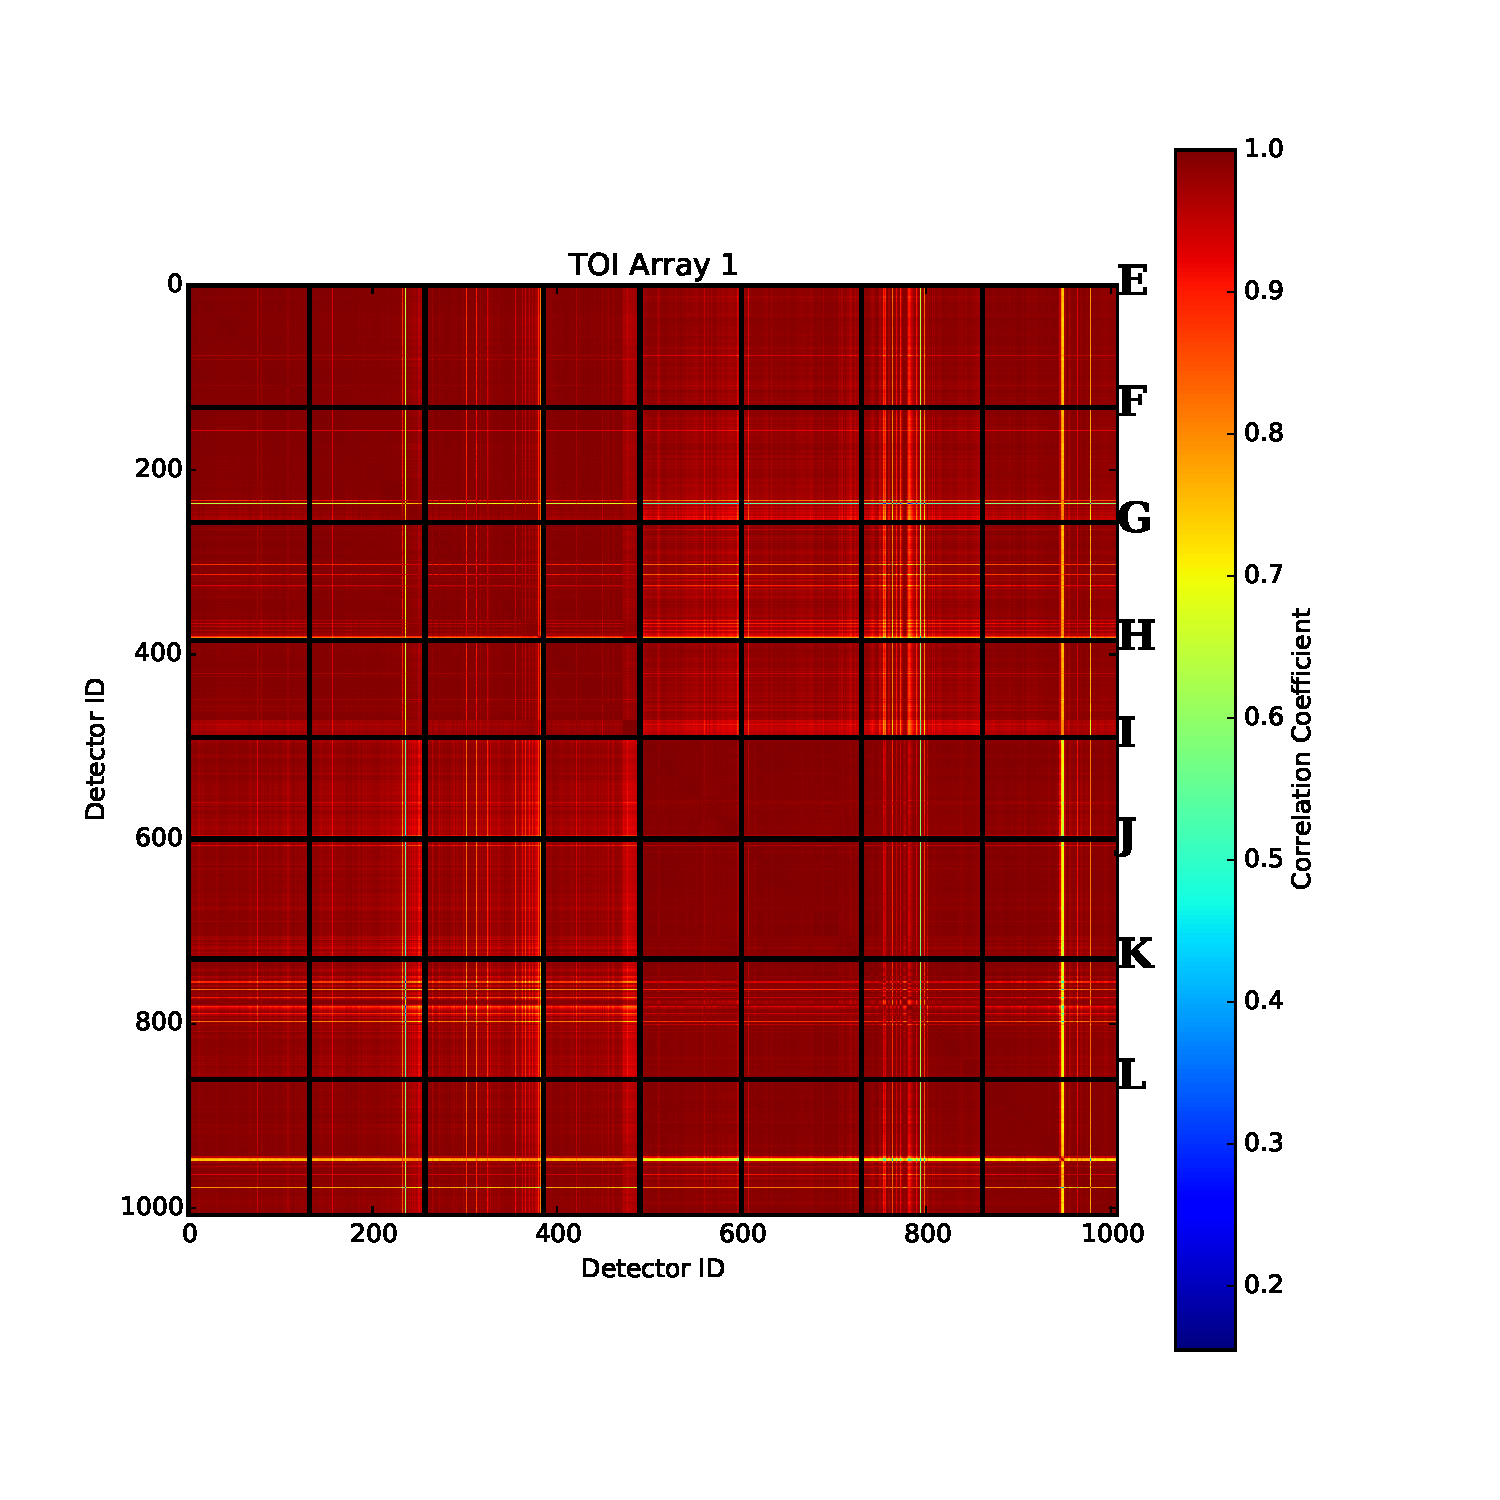
\includegraphics[width=0.3\textwidth]{Figures/NoiseTests/corrmat_TOI_array_1_20170228s151.pdf}
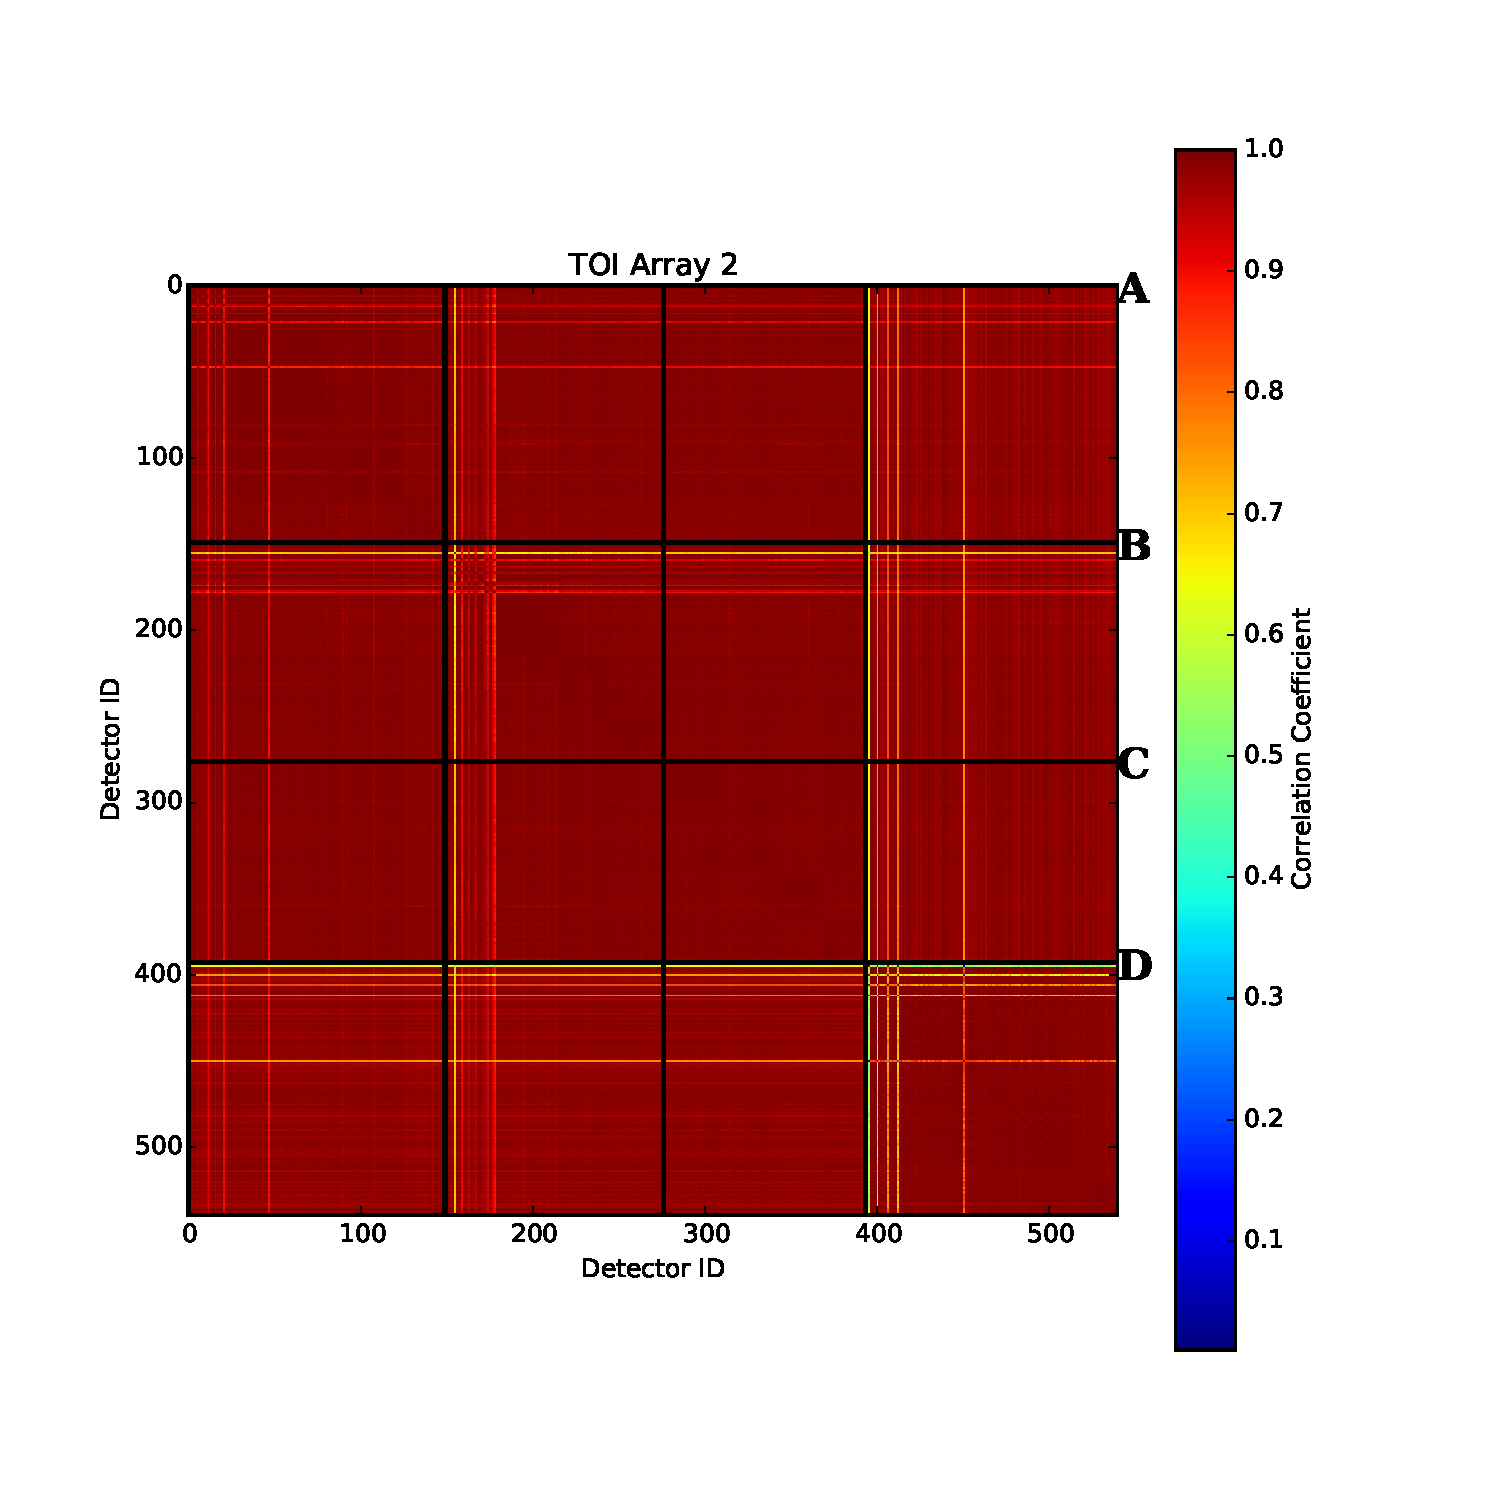
\includegraphics[width=0.3\textwidth]{Figures/NoiseTests/corrmat_TOI_array_2_20170228s151.pdf}
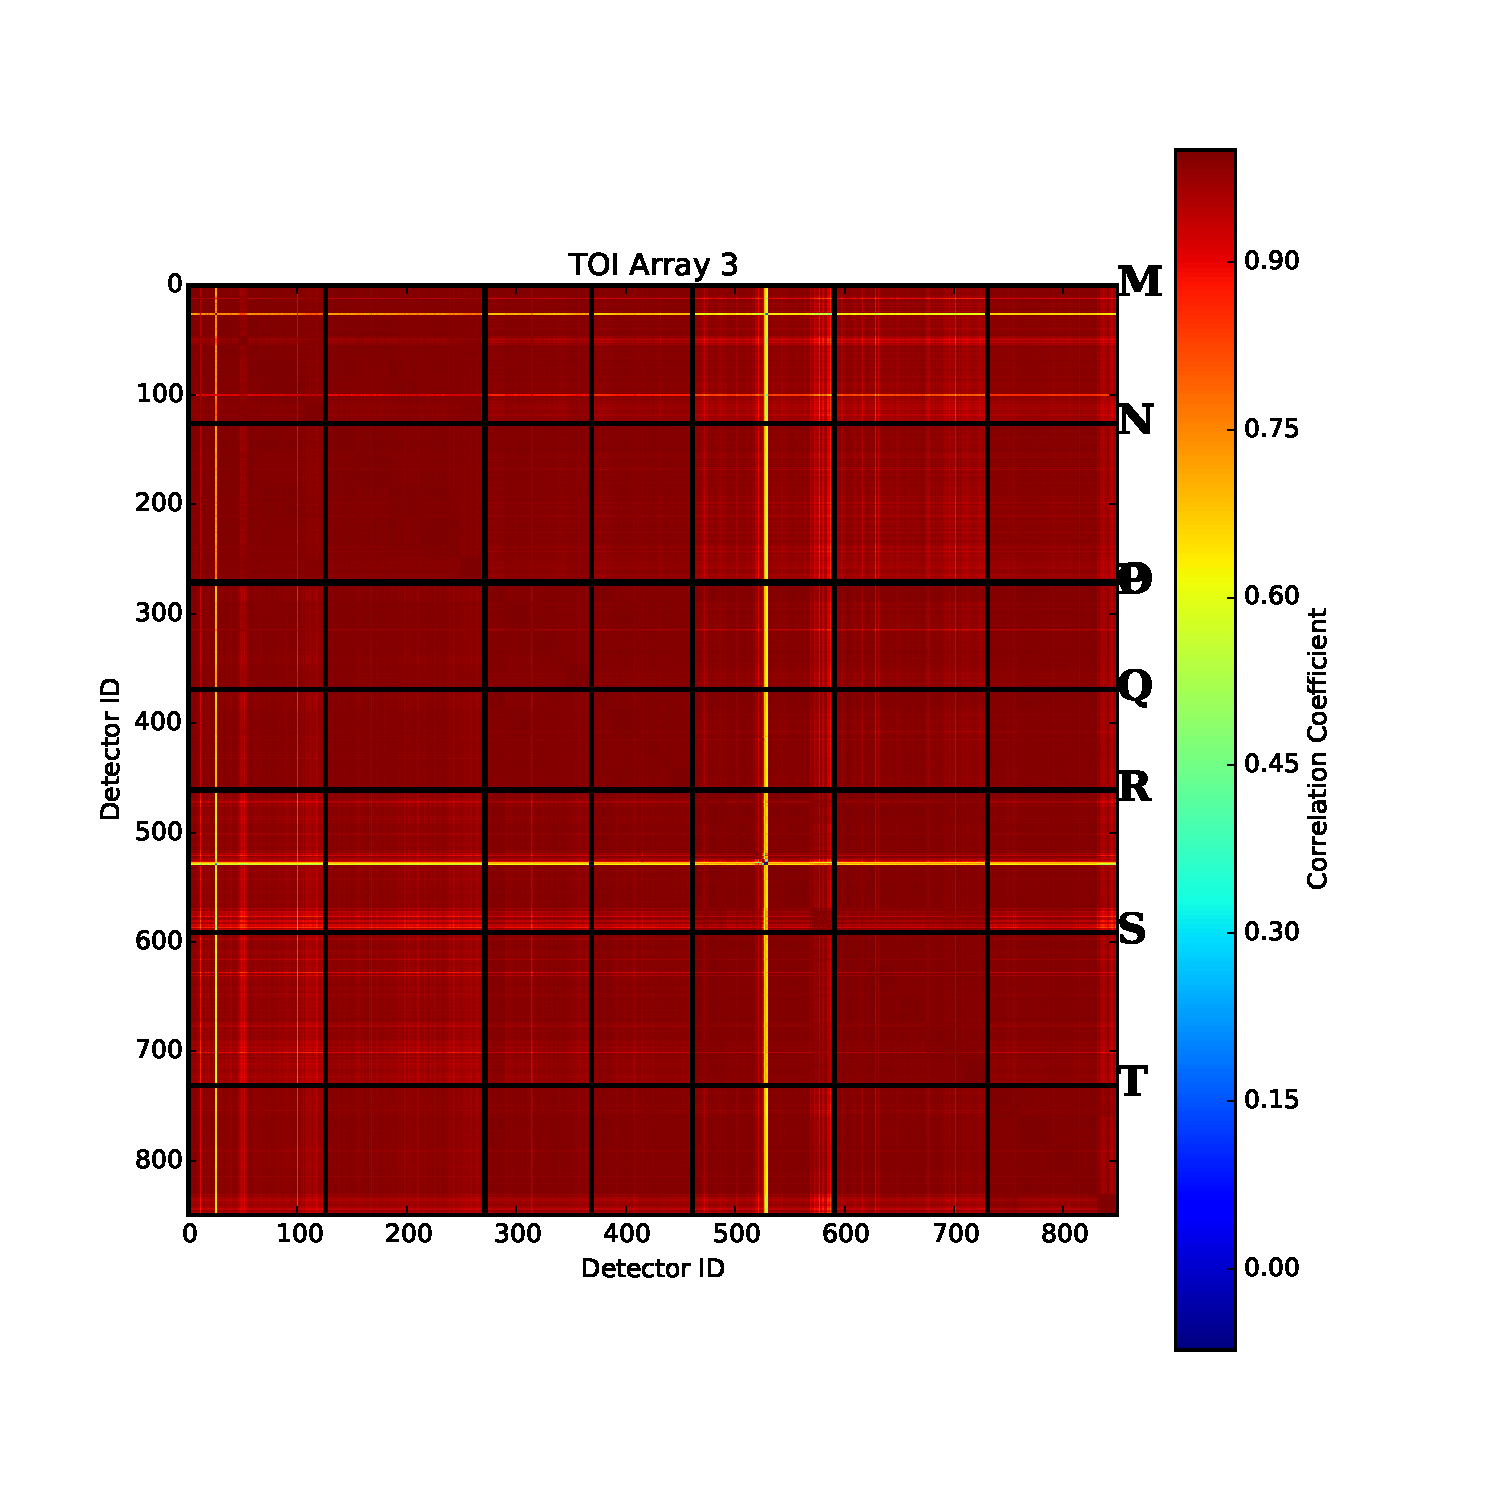
\includegraphics[width=0.3\textwidth]{Figures/NoiseTests/corrmat_TOI_array_3_20170228s151.pdf}
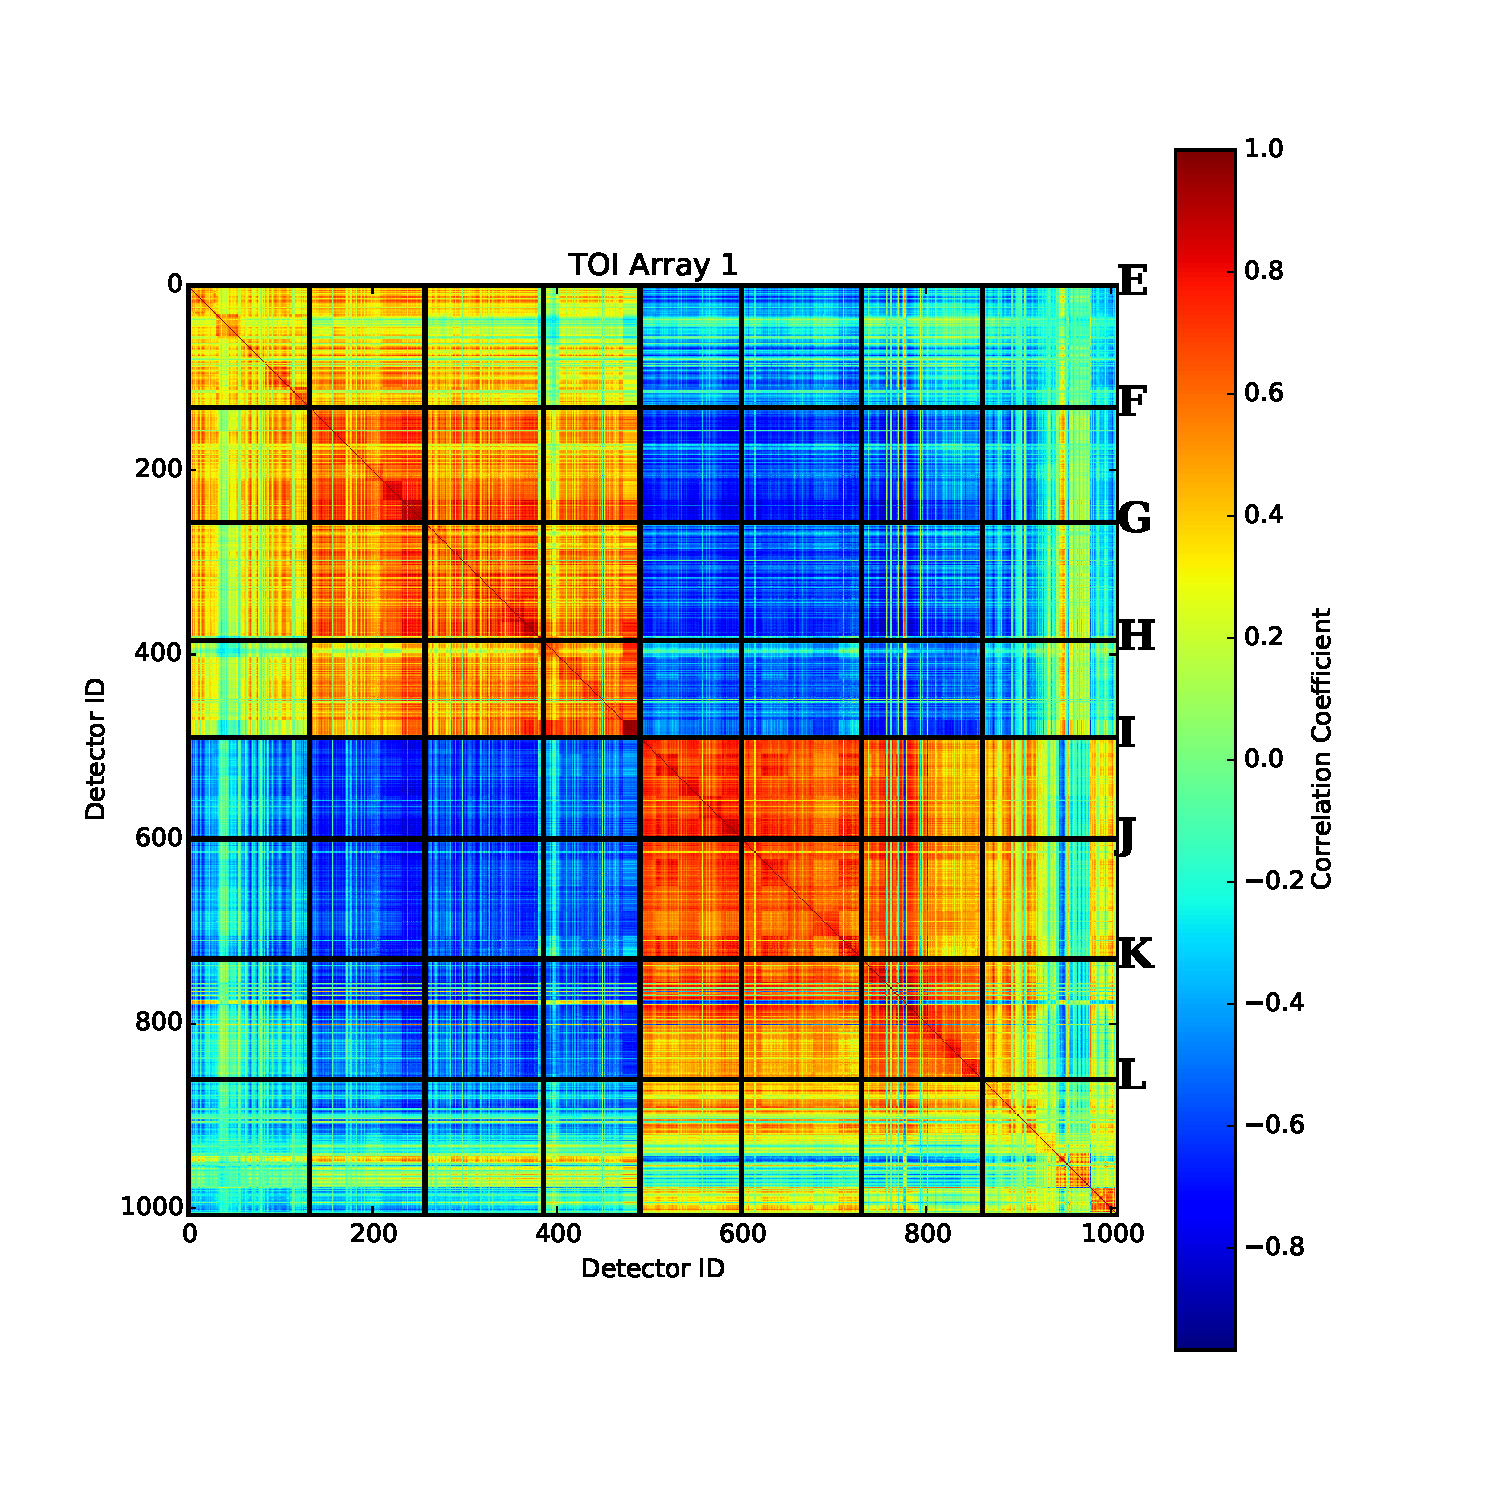
\includegraphics[width=0.3\textwidth]{Figures/NoiseTests/corrmat_TOI_CM_array_1_20170228s151.pdf}
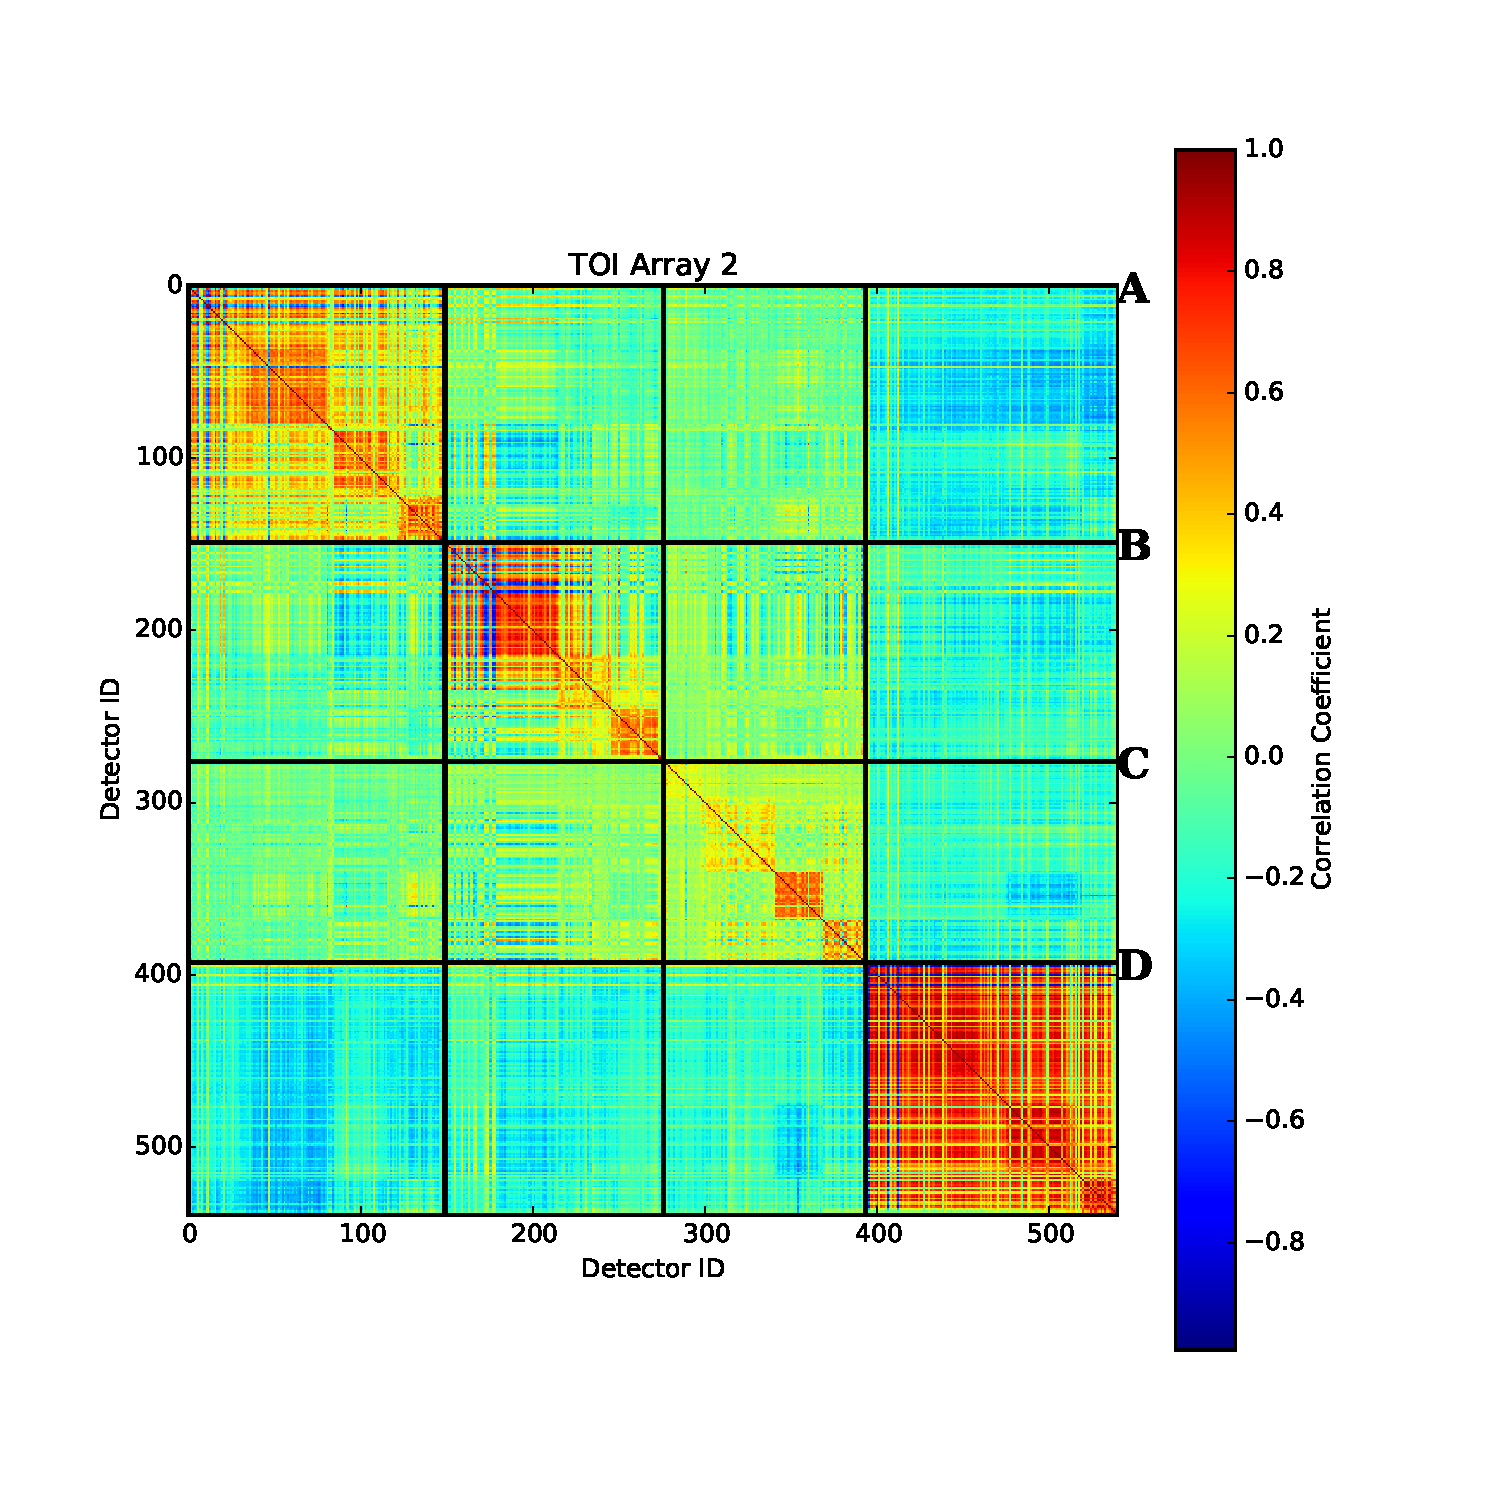
\includegraphics[width=0.3\textwidth]{Figures/NoiseTests/corrmat_TOI_CM_array_2_20170228s151.pdf}
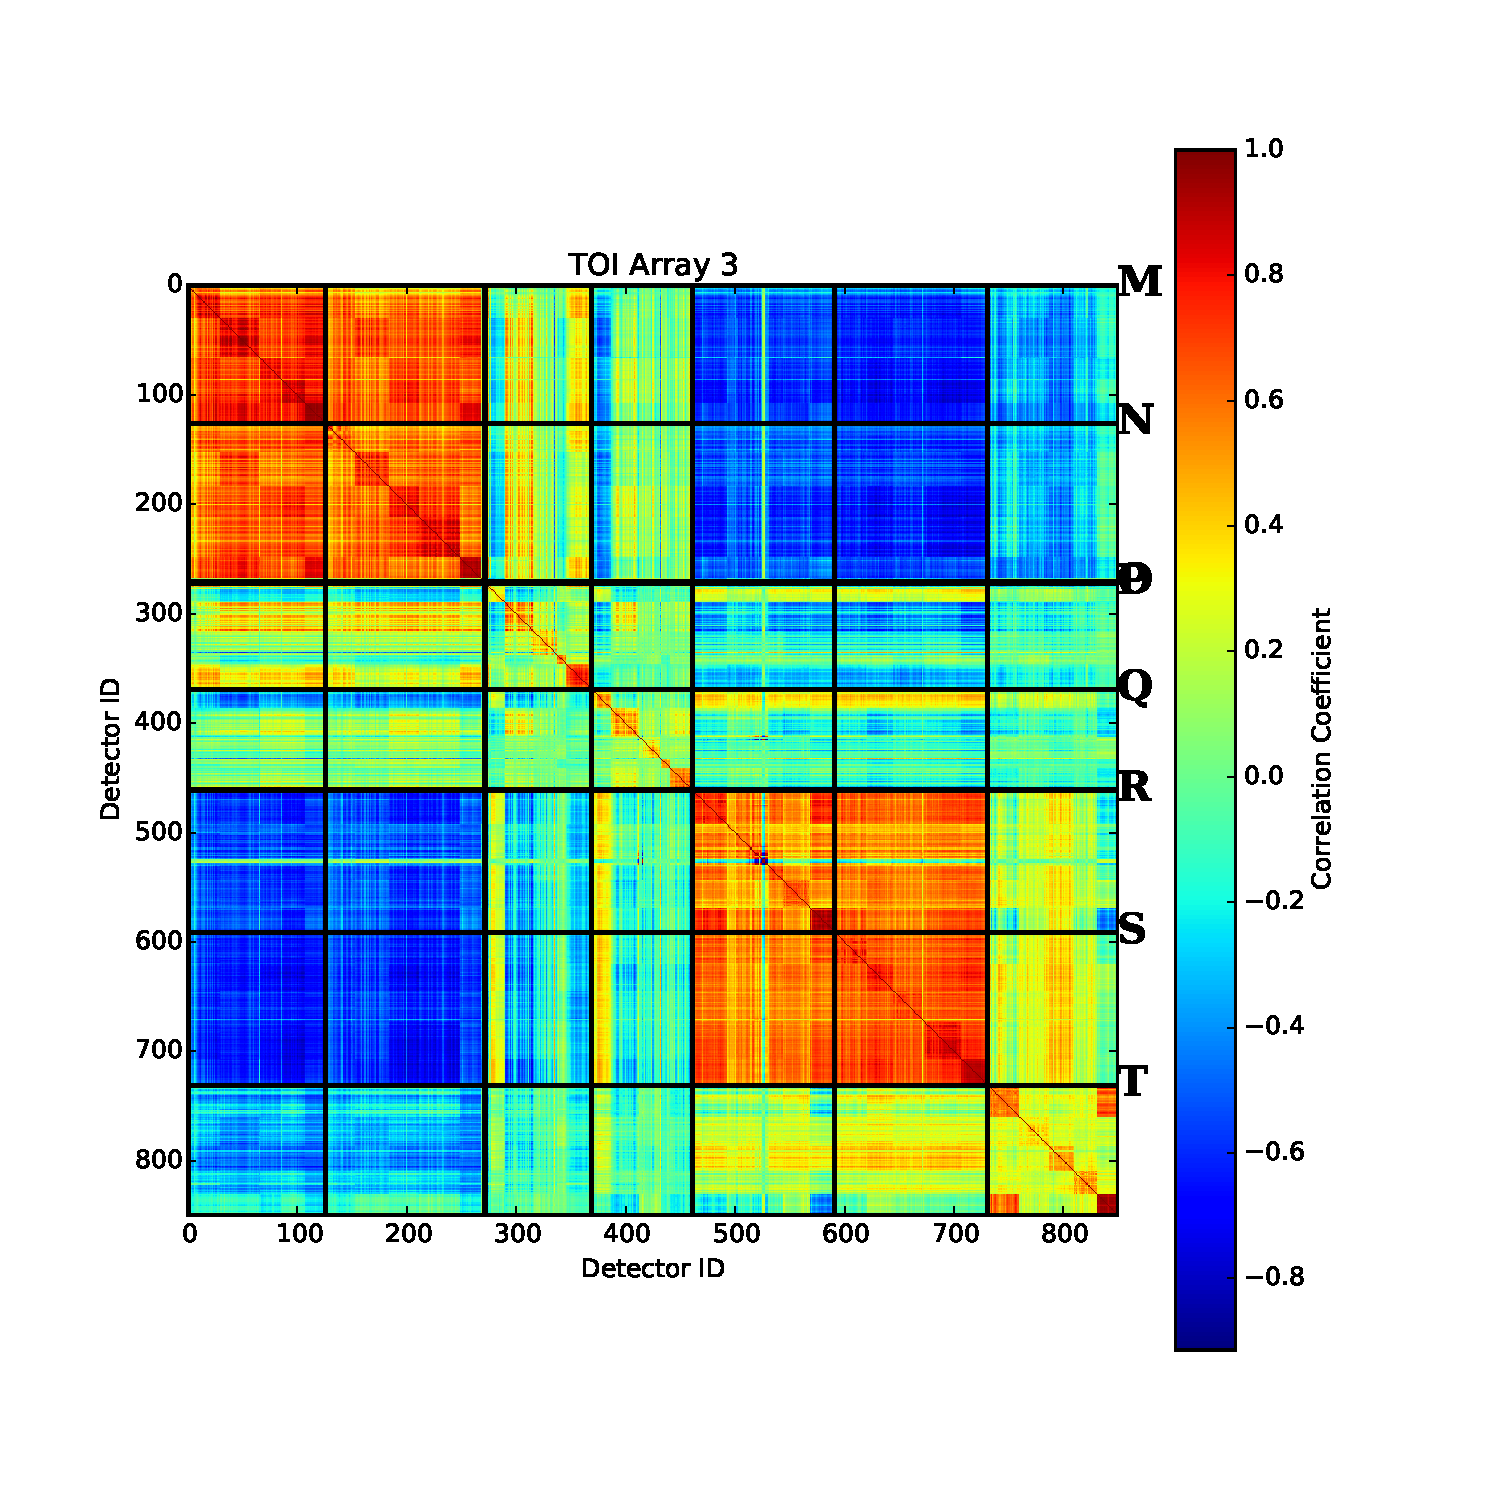
\includegraphics[width=0.3\textwidth]{Figures/NoiseTests/corrmat_TOI_CM_array_3_20170228s151.pdf}
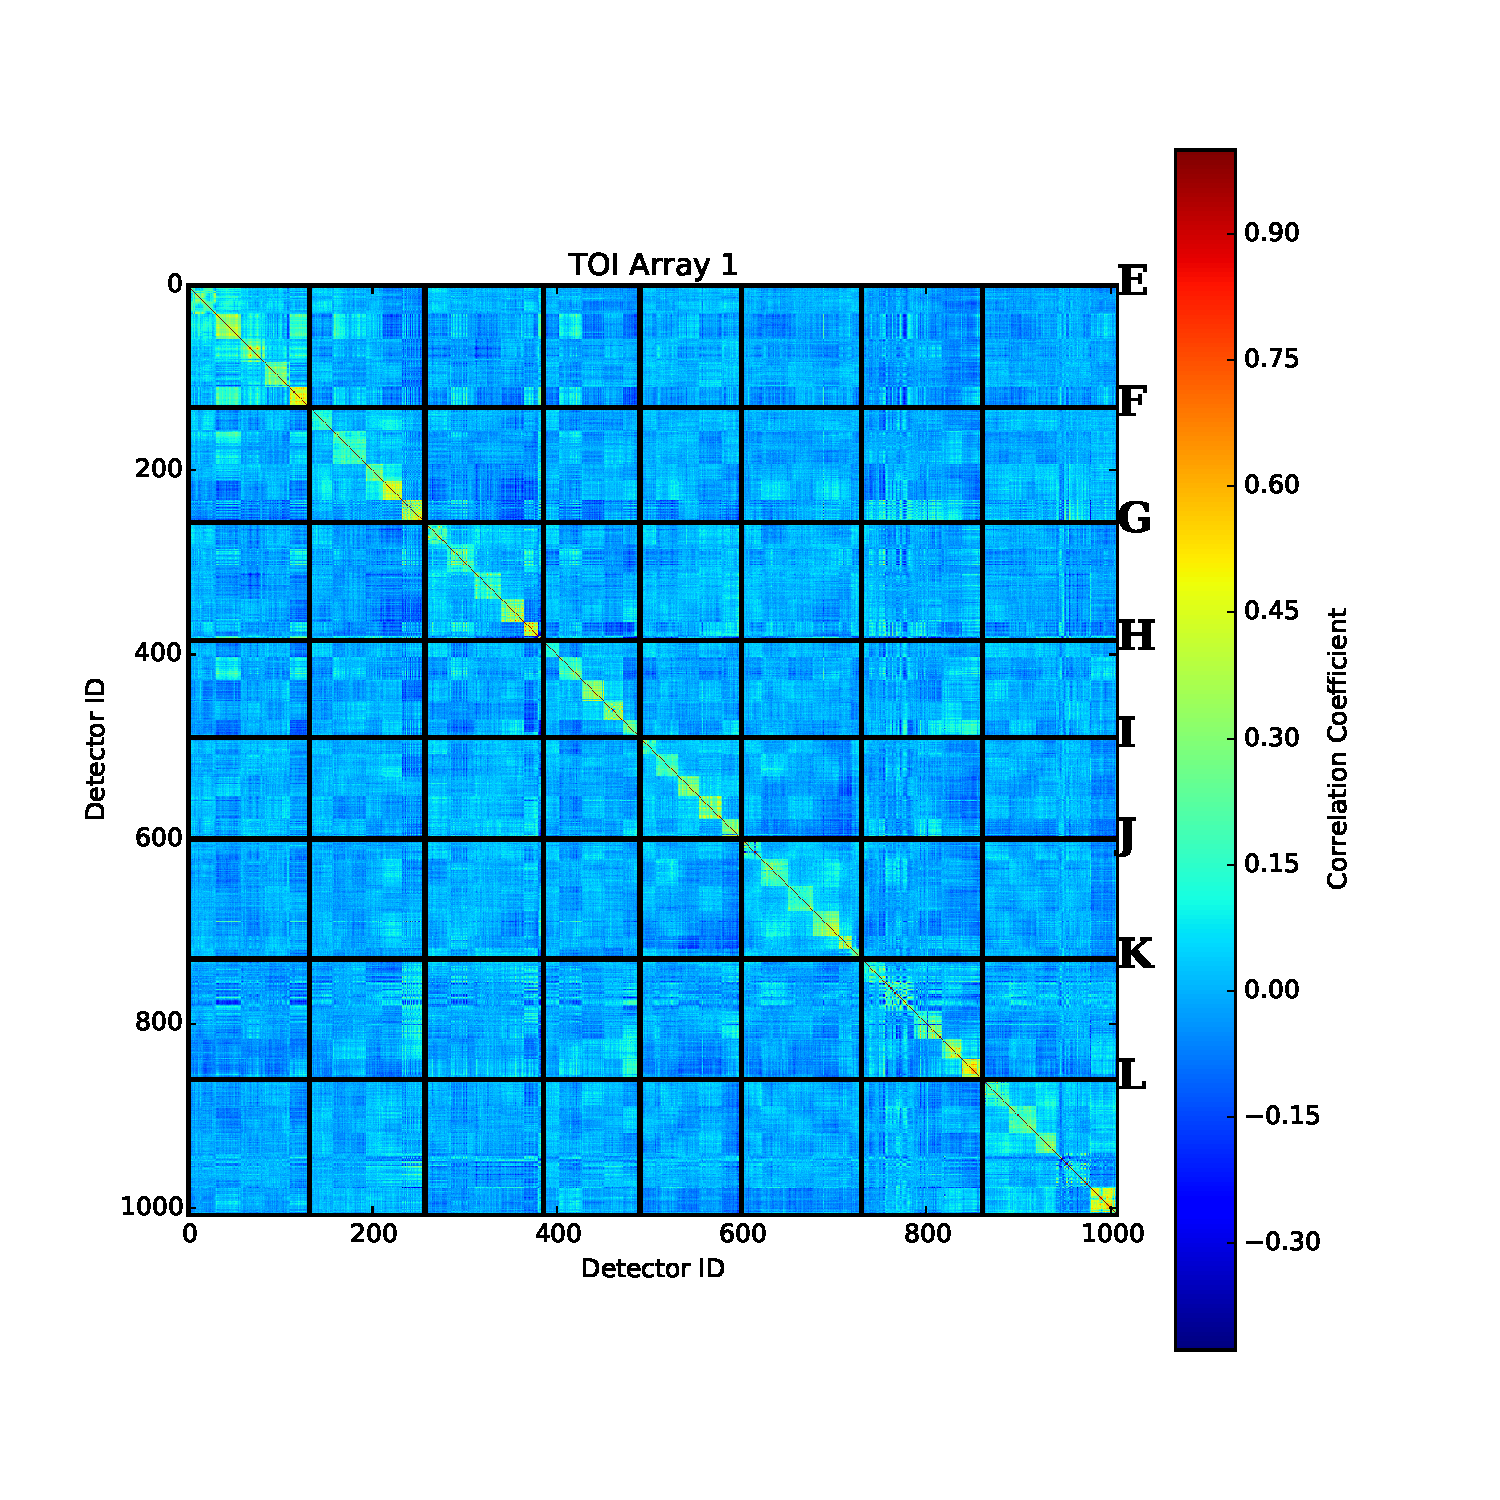
\includegraphics[width=0.3\textwidth]{Figures/NoiseTests/corrmat_TOI_PCA_array_1_20170228s151.pdf}
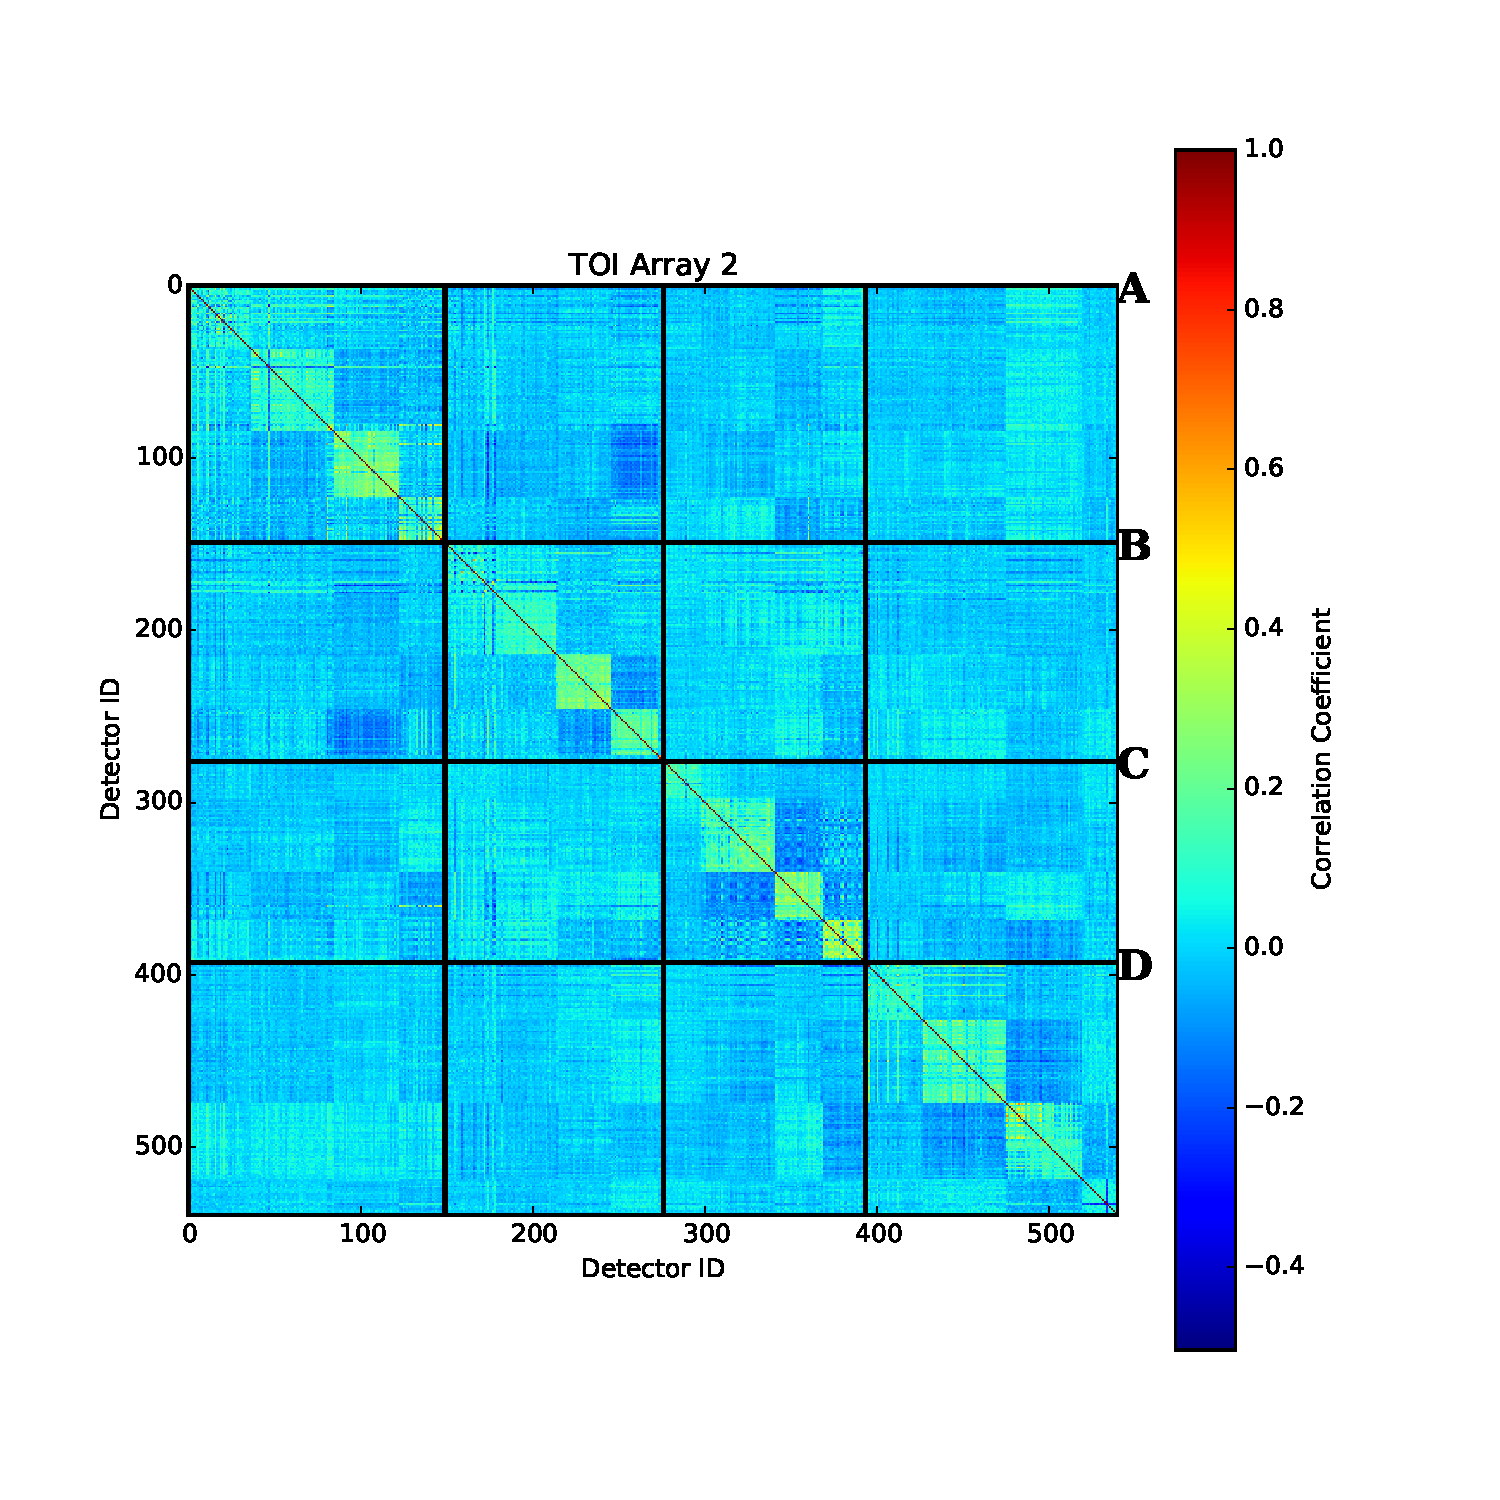
\includegraphics[width=0.3\textwidth]{Figures/NoiseTests/corrmat_TOI_PCA_array_2_20170228s151.pdf}
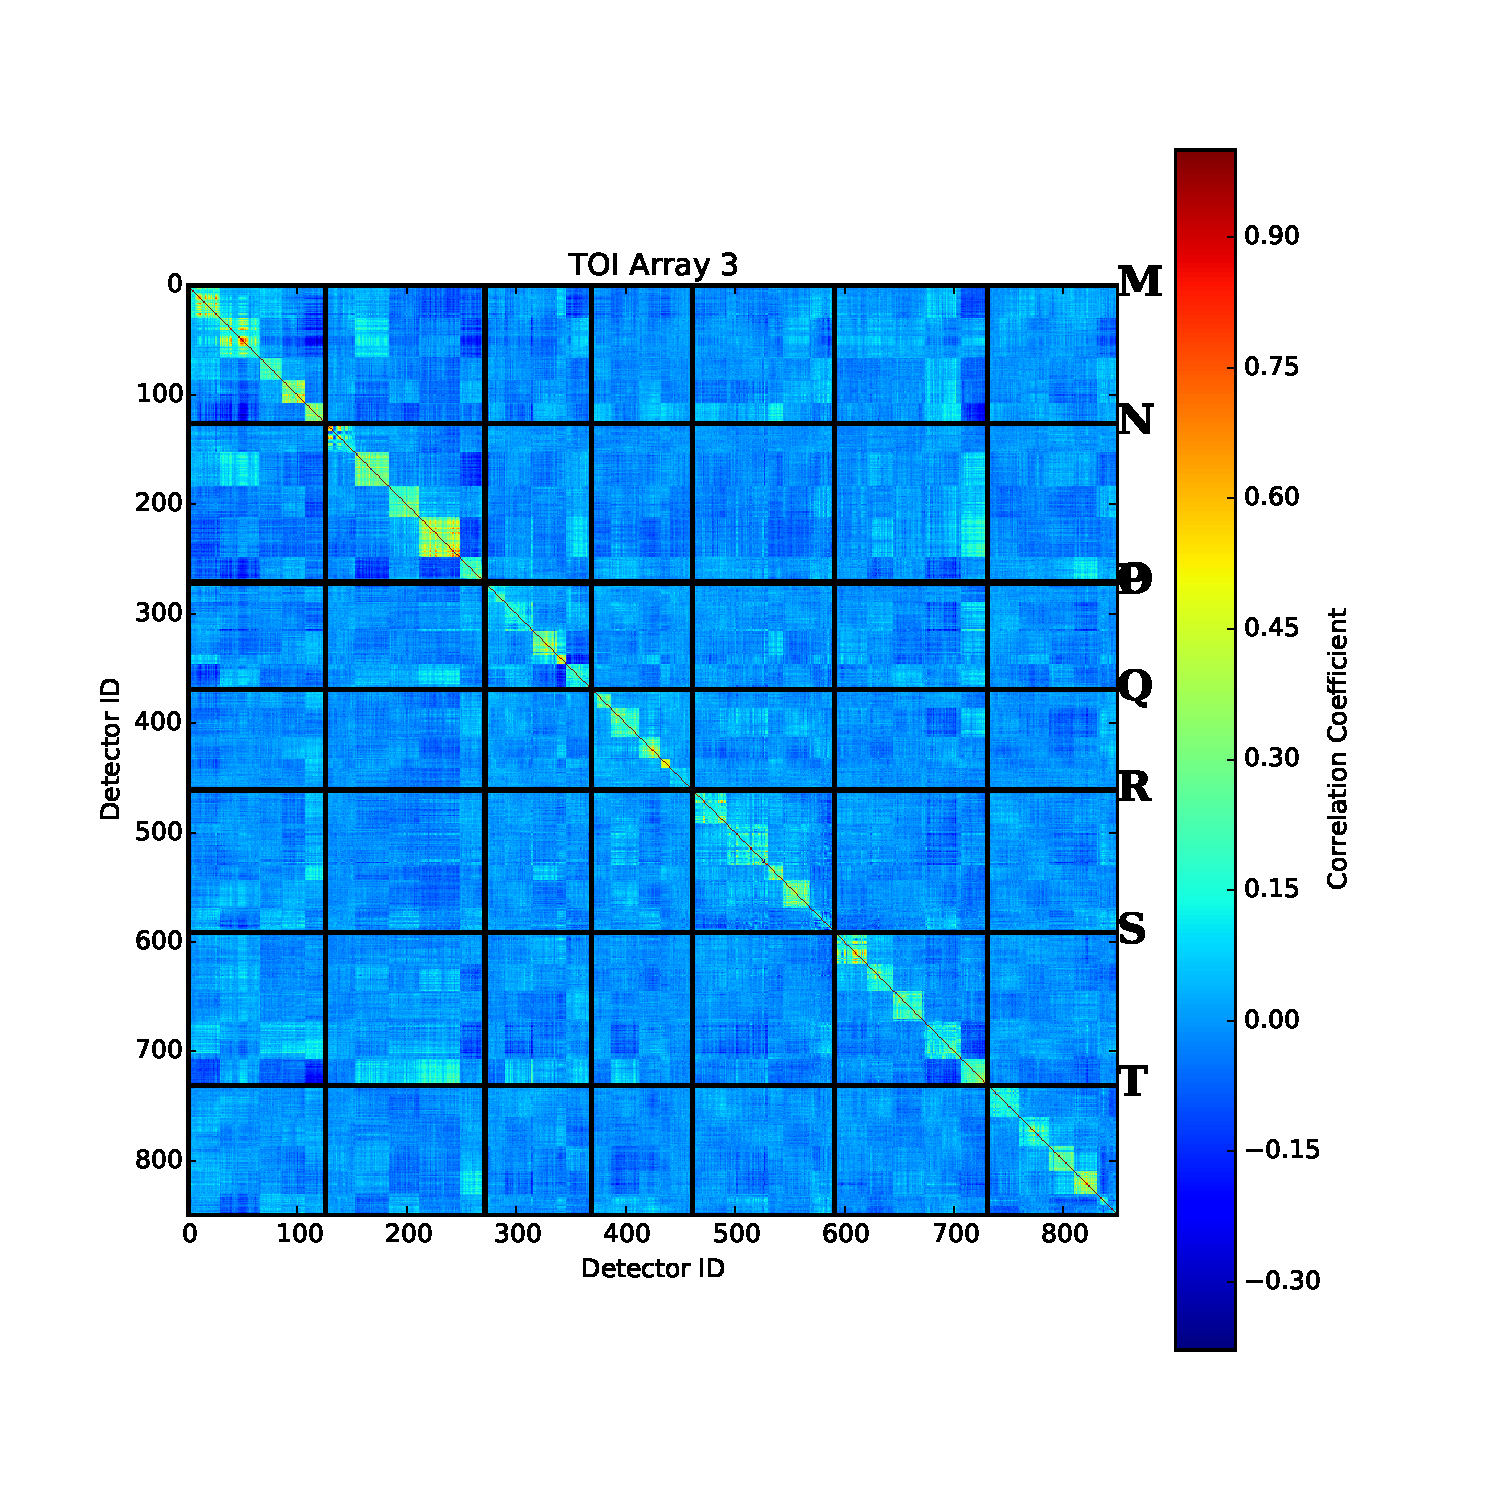
\includegraphics[width=0.3\textwidth]{Figures/NoiseTests/corrmat_TOI_PCA_array_3_20170228s151.pdf}
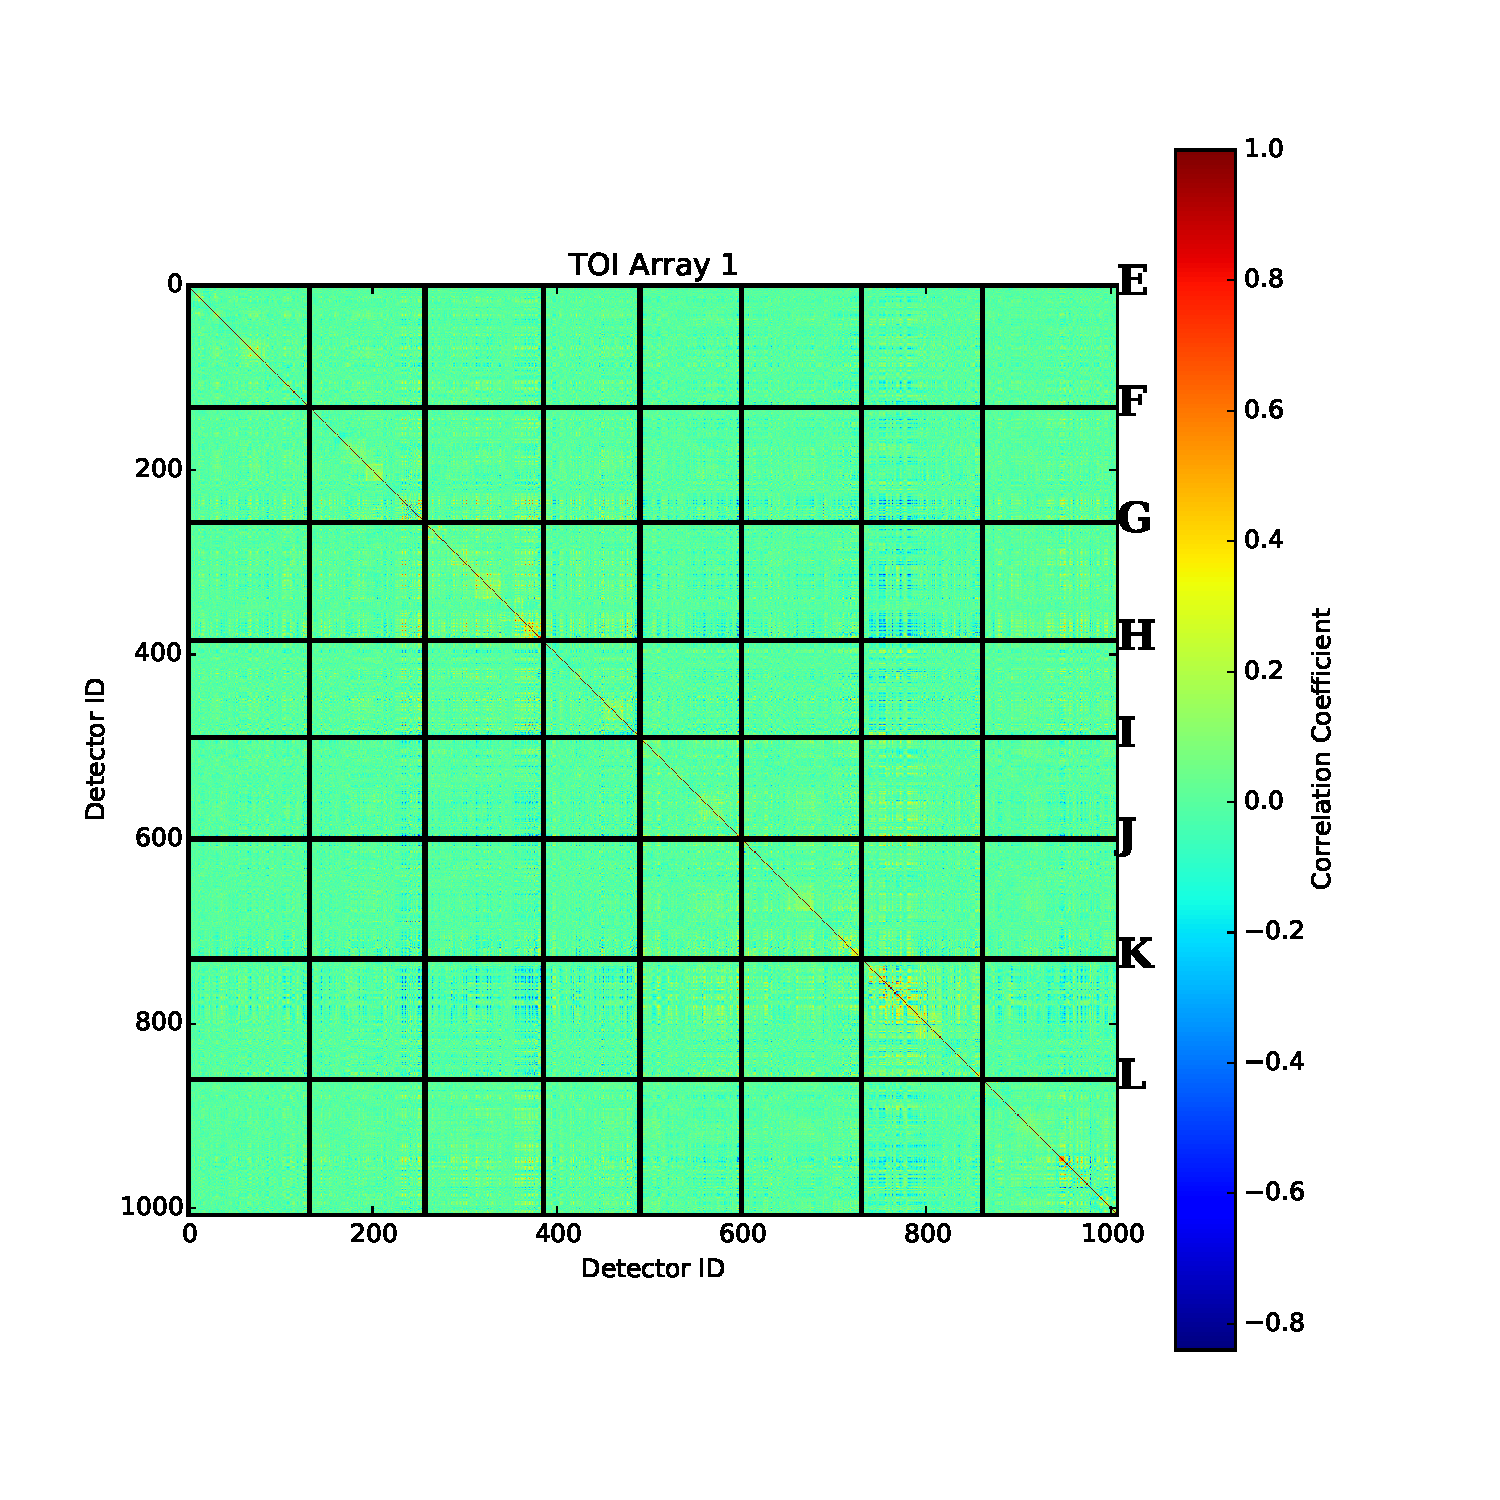
\includegraphics[width=0.3\textwidth]{Figures/NoiseTests/corrmat_TOI_BCP_array_1_20170228s151.pdf}
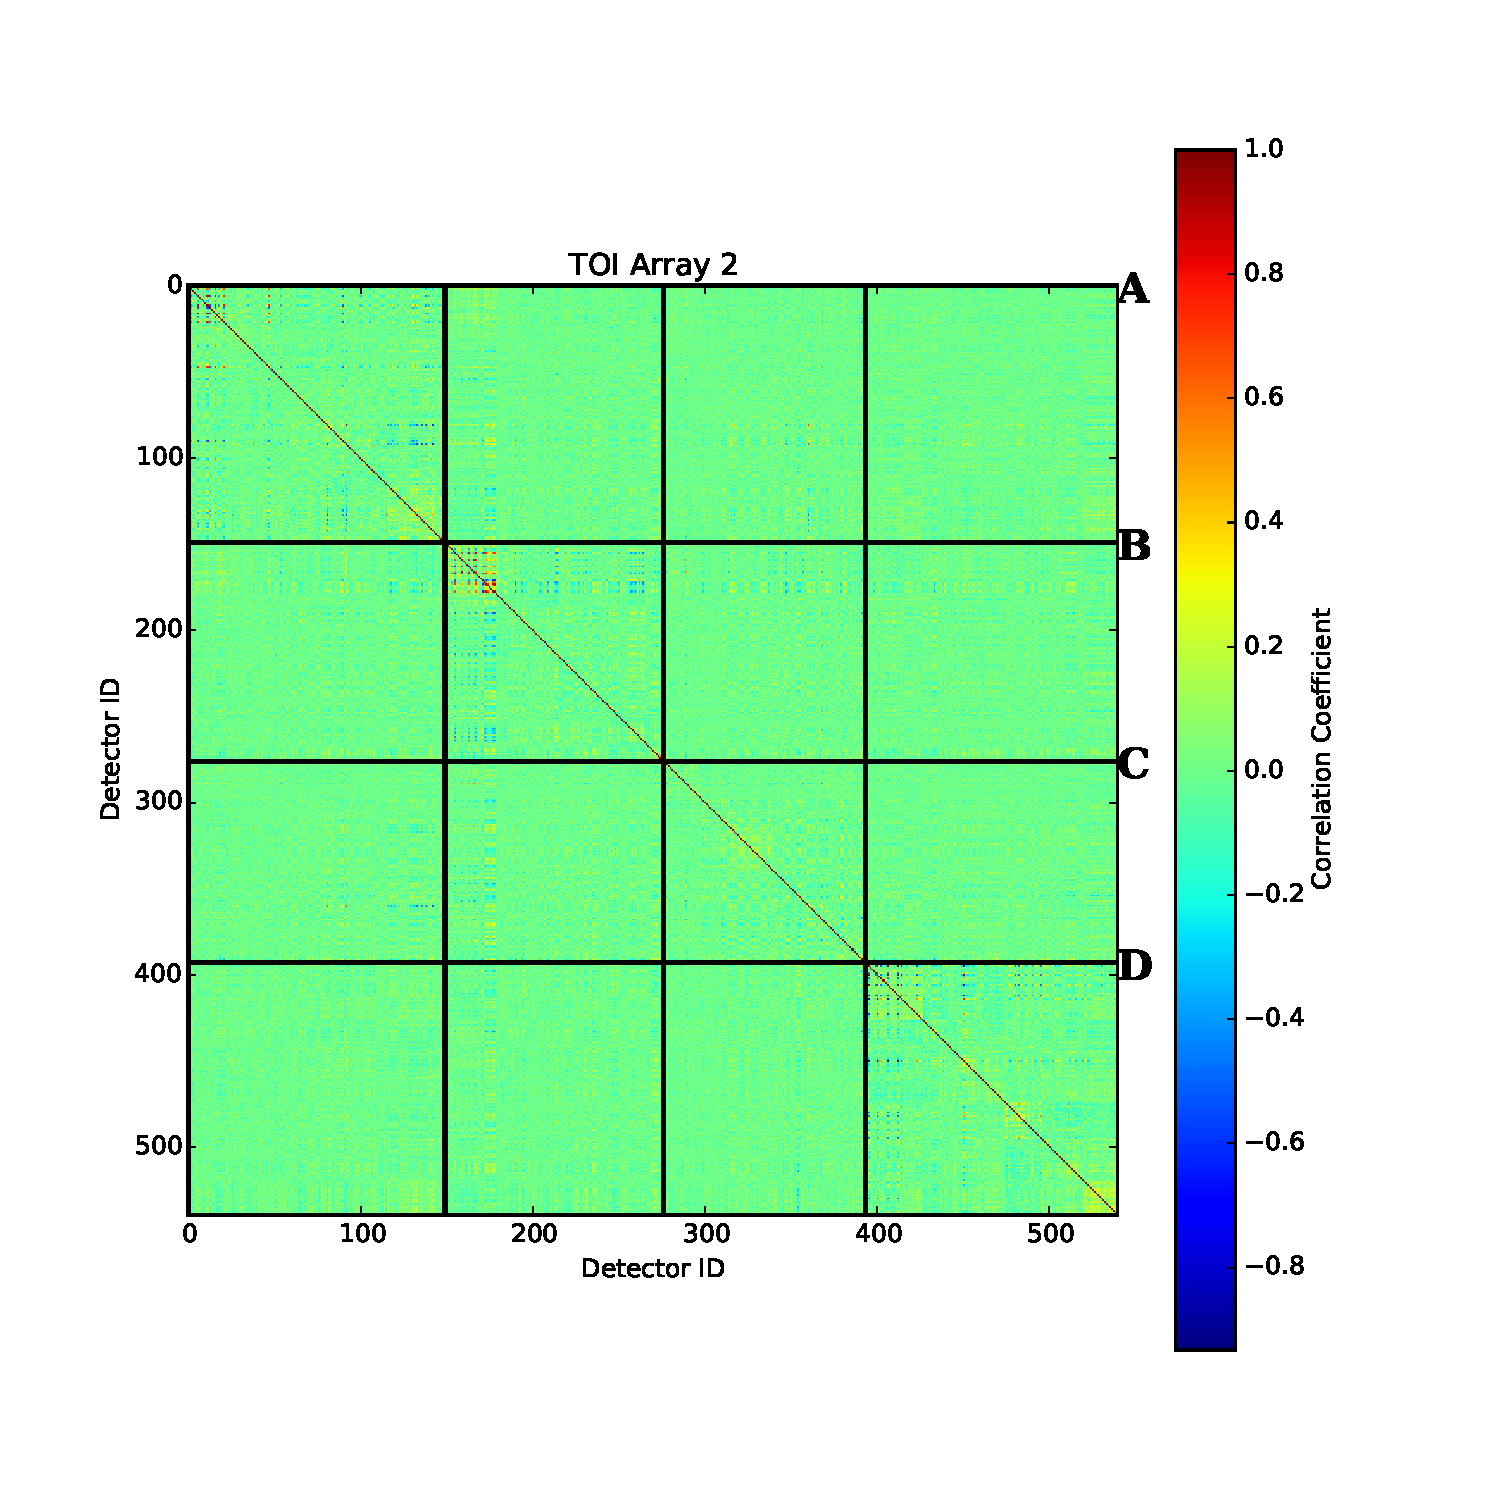
\includegraphics[width=0.3\textwidth]{Figures/NoiseTests/corrmat_TOI_BCP_array_2_20170228s151.pdf}
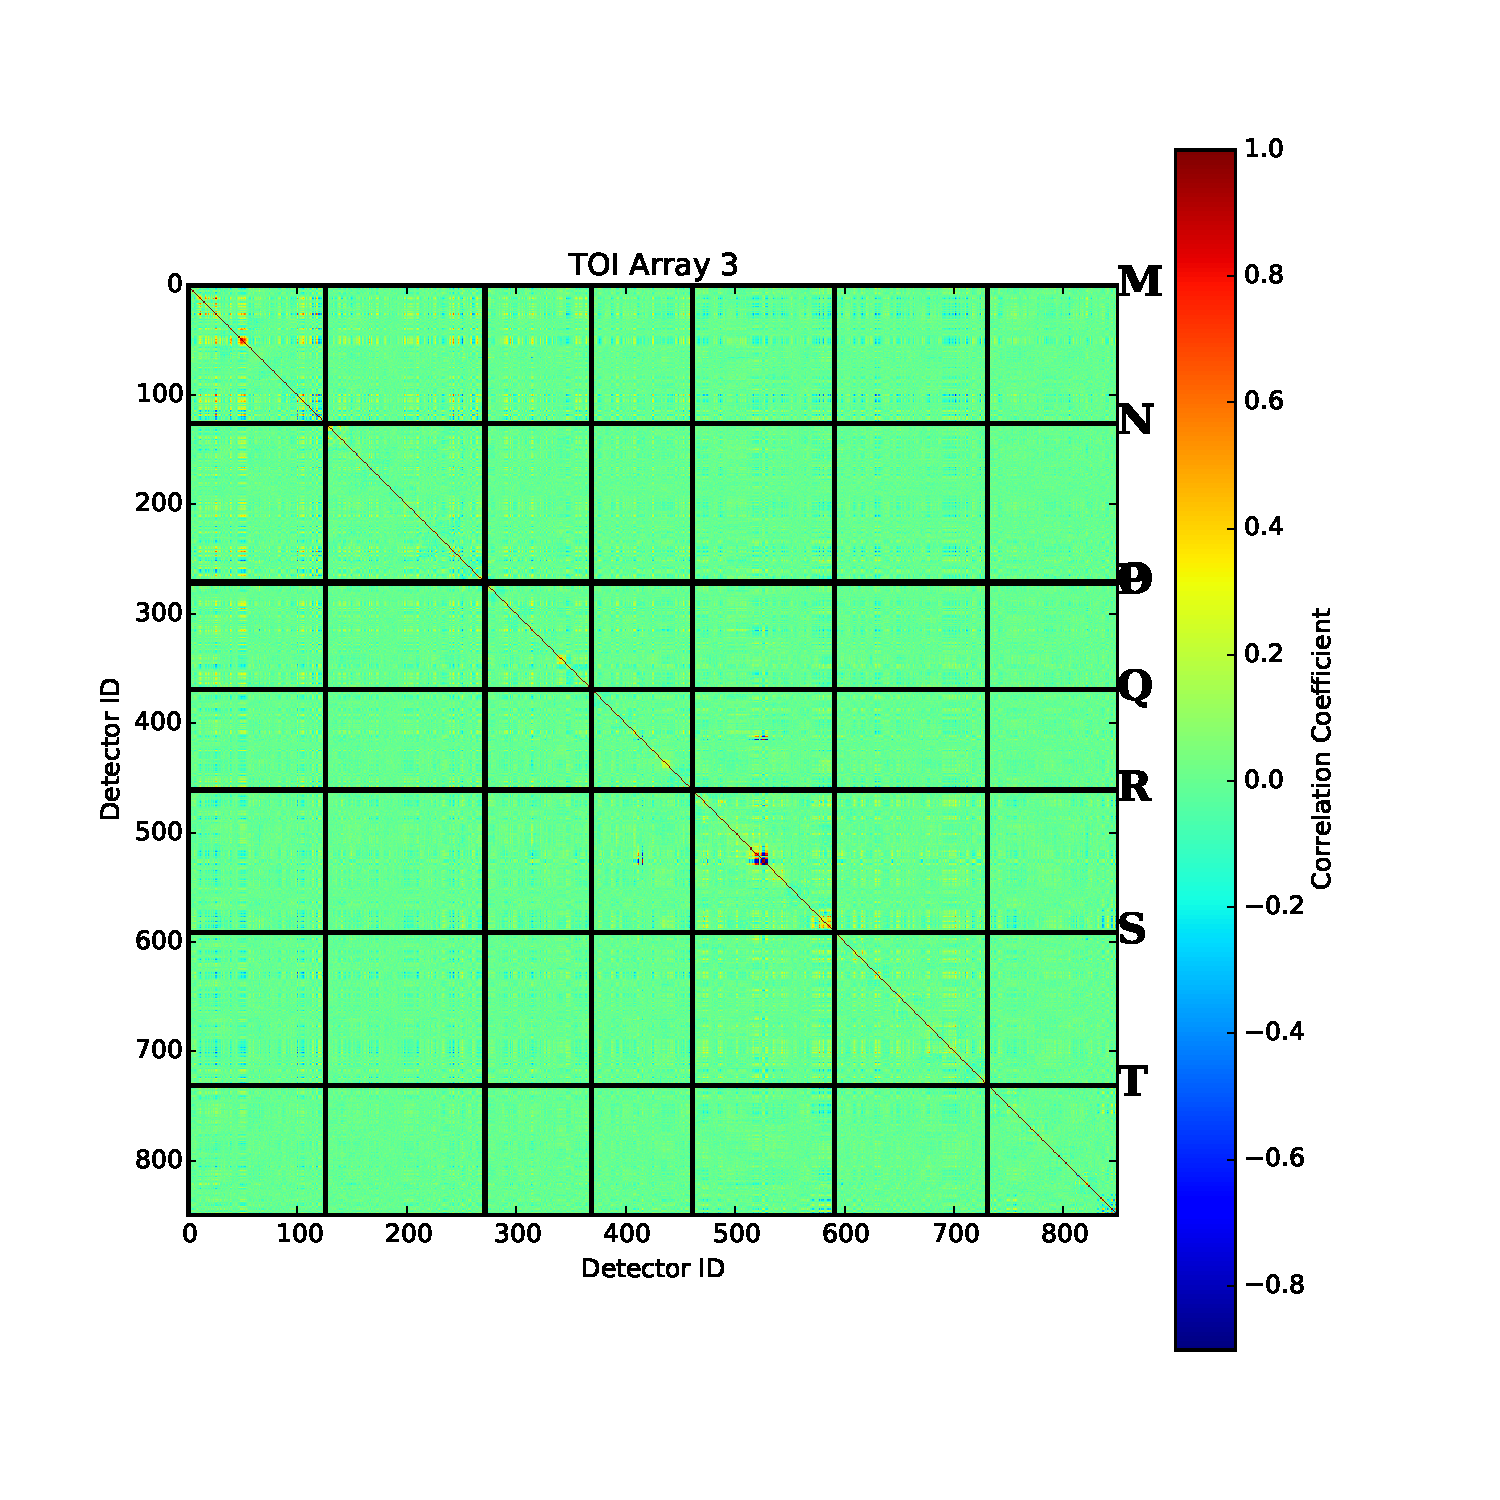
\includegraphics[width=0.3\textwidth]{Figures/NoiseTests/corrmat_TOI_BCP_array_3_20170228s151.pdf}
\end{center}
\caption[KID-to-KID correlation matrices]{\emph{From left to right:} TOI correlation
  matrices for the three NIKA2 arrays (A1, A2, and A3) for scan
  20170228s150. From top to bottom we present the correlation of the raw data,
  after CM, PCA and MCP decorrelation methods. \label{corrmatrix}}
\end{figure}

As presented on Fig.~\ref{fig:nika_toi}, the atmosphere and the electronic noise
combine into a large low frequency component that we want to eliminate as much
as possible. Most of the atmospheric component is common to all KIDs, which is
expected because the telescope is a $30\,\rm{m}$ dish and therefore
has a \todo{Carsten comments: XXXX near field of XXXXX m $->$
  effective collecting area of $170~\rm{m}^2$ at 1.2~mm ?}. 

On Fig.~\ref{fig:nika_toi}, the planet Uranus is visible in the TOIs and serves as
guide to both the noise relative amplitude and the discussion about TOI
processing in the following. On Fig.~\ref{corrmatrix}, we take a scan on Pluto
where the signal is negligible compared to noise on the timescale of a scan to
focus on the noise properties. We present the KID to KID timeline correlation
matrices for the three arrays, either before any data reduction or with
different estimates of the low frequency component:

\begin{itemize}
\item {\bf Common Mode decorrelation (CM)}. We use all detectors of the same
  array to build an average low frequency component nicknamed \emph{common
    mode}. This mode is then linearly regressed and subtracted from each KID
  timeline. In this method, the \emph{common mode} at time $t$ is the median of
  all KIDs at this time $t$.

\item {\bf Principal Component Analysis (PCA)}. For each NIKA2 array
  independently we decompose the covariance matrix in principal components. From
  those we derive up to 10 independent templates corresponding to the largest
  eigenvalues \todo{that we subtract from the TOIs XXX TBC XXXX}.

\item {\bf Most correlated pixels (\cmoneb)}. For each detector in a given array we
  identify the detectors that are most correlated to it (a minimum of
  15). Using those detectors we compute a common mode like in method CM but with
  more refinements to be valid even on bright sources (see below).
\end{itemize}

As expected the raw data
noise correlation is dominated by atmospheric noise and we observe full
correlation between detectors but for badly behaving detectors which are removed
from the analysis. Significant residual correlation and anti-correlation is
observed after CM decorrelation. This is both due to spatial changes in the
atmospheric emission (overall residuals) and to instrumental and electronic
noise characteristics (correlation blocks that can be associated to electronic
boxes).  The PCA decorrelation leads to approximately block-diagonal correlation
matrices. These observed blocks in the correlation matrix can be associated to
first order to the different sub-bands in each of the electronic boxes. In the
case of the MCP decorrelation, for which only those pixels highly correlated to
the pixel of interest are used, we observe that the correlation matrix is more
diagonal as in the two other derivations of the common mode.

\begin{figure}[ht!] % Inline image example
\begin{center}
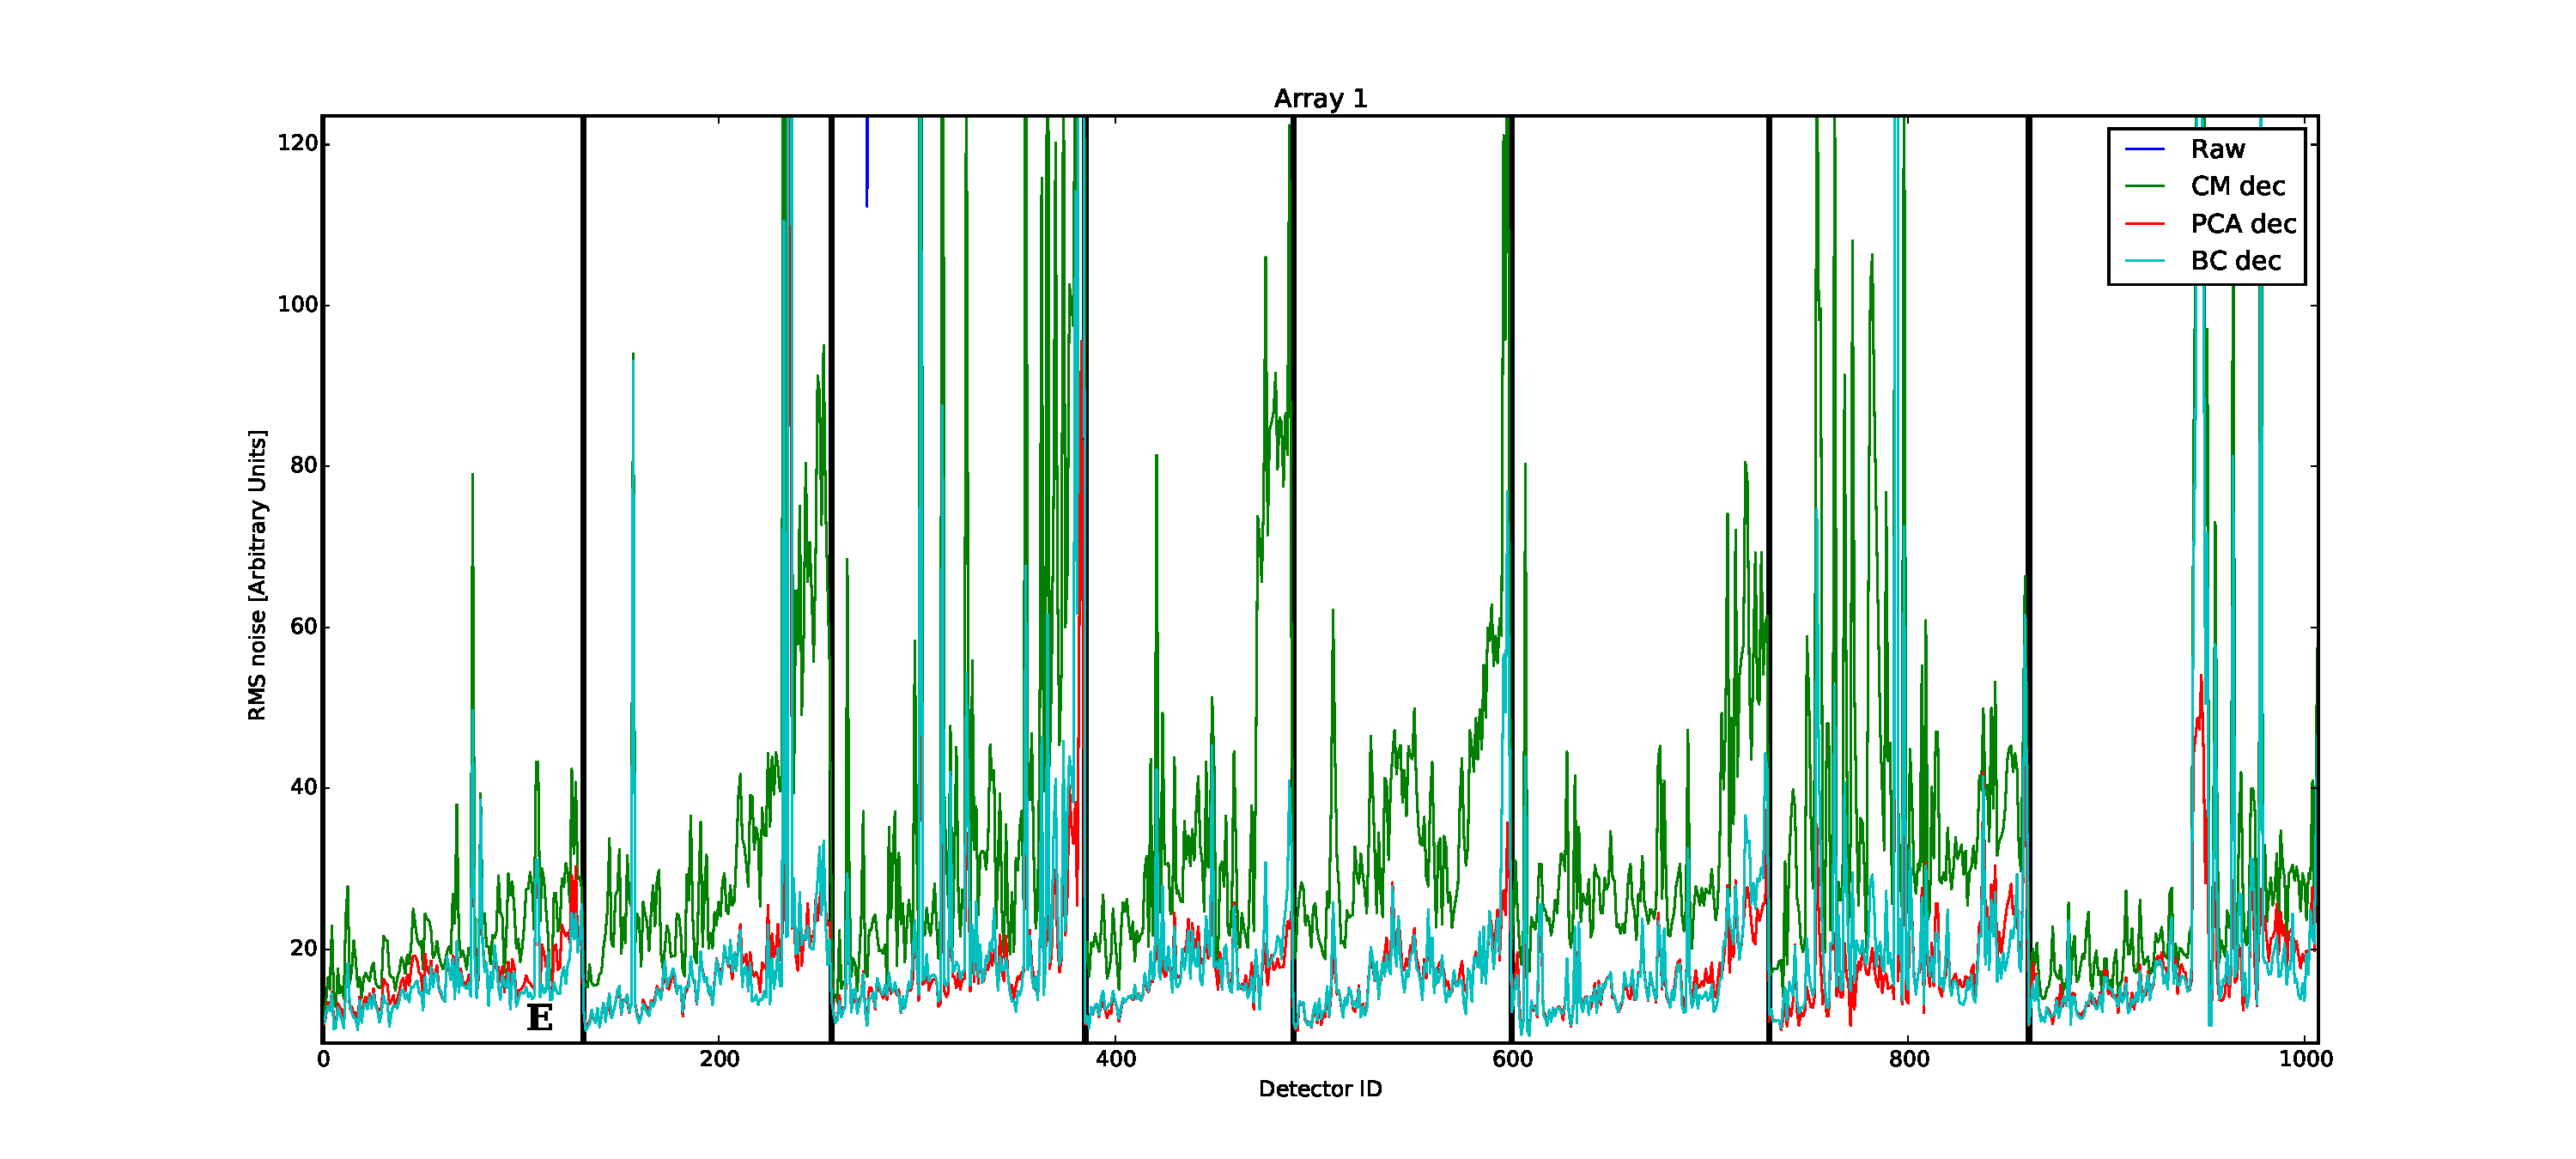
\includegraphics[clip=true, trim={0.5cm, 0, 0, 0.6cm},width=0.32\textwidth]{Figures/NoiseTests/rms_TOI_array_1_20170228s151.pdf}
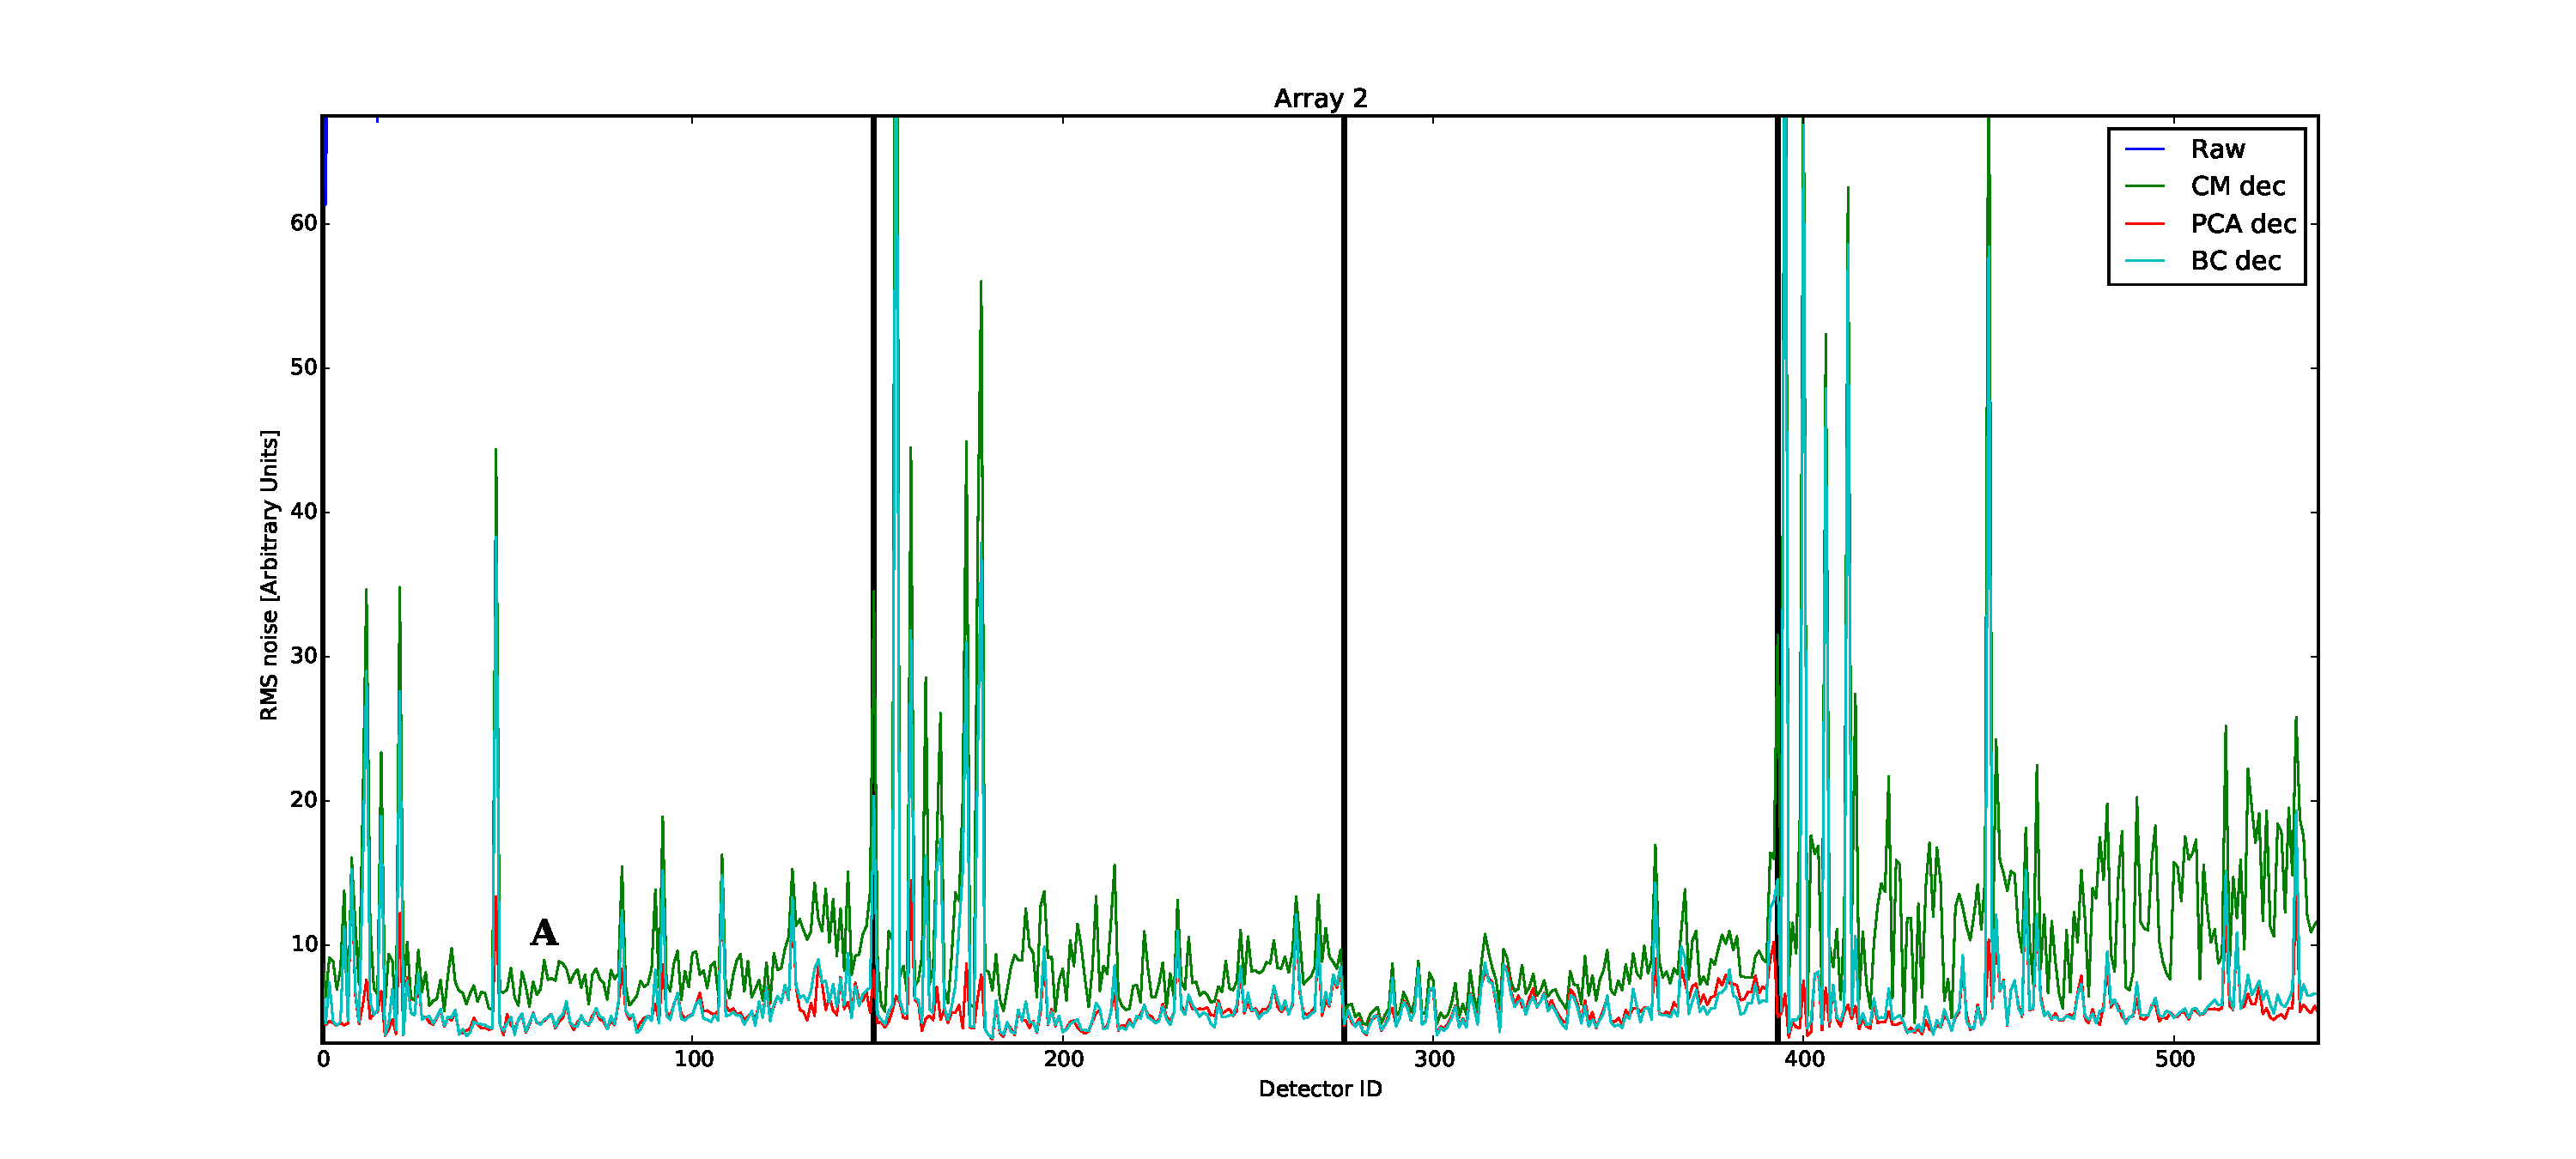
\includegraphics[clip=true, trim={0.5cm, 0, 0, 0.6cm},width=0.32\textwidth]{Figures/NoiseTests/rms_TOI_array_2_20170228s151.pdf}
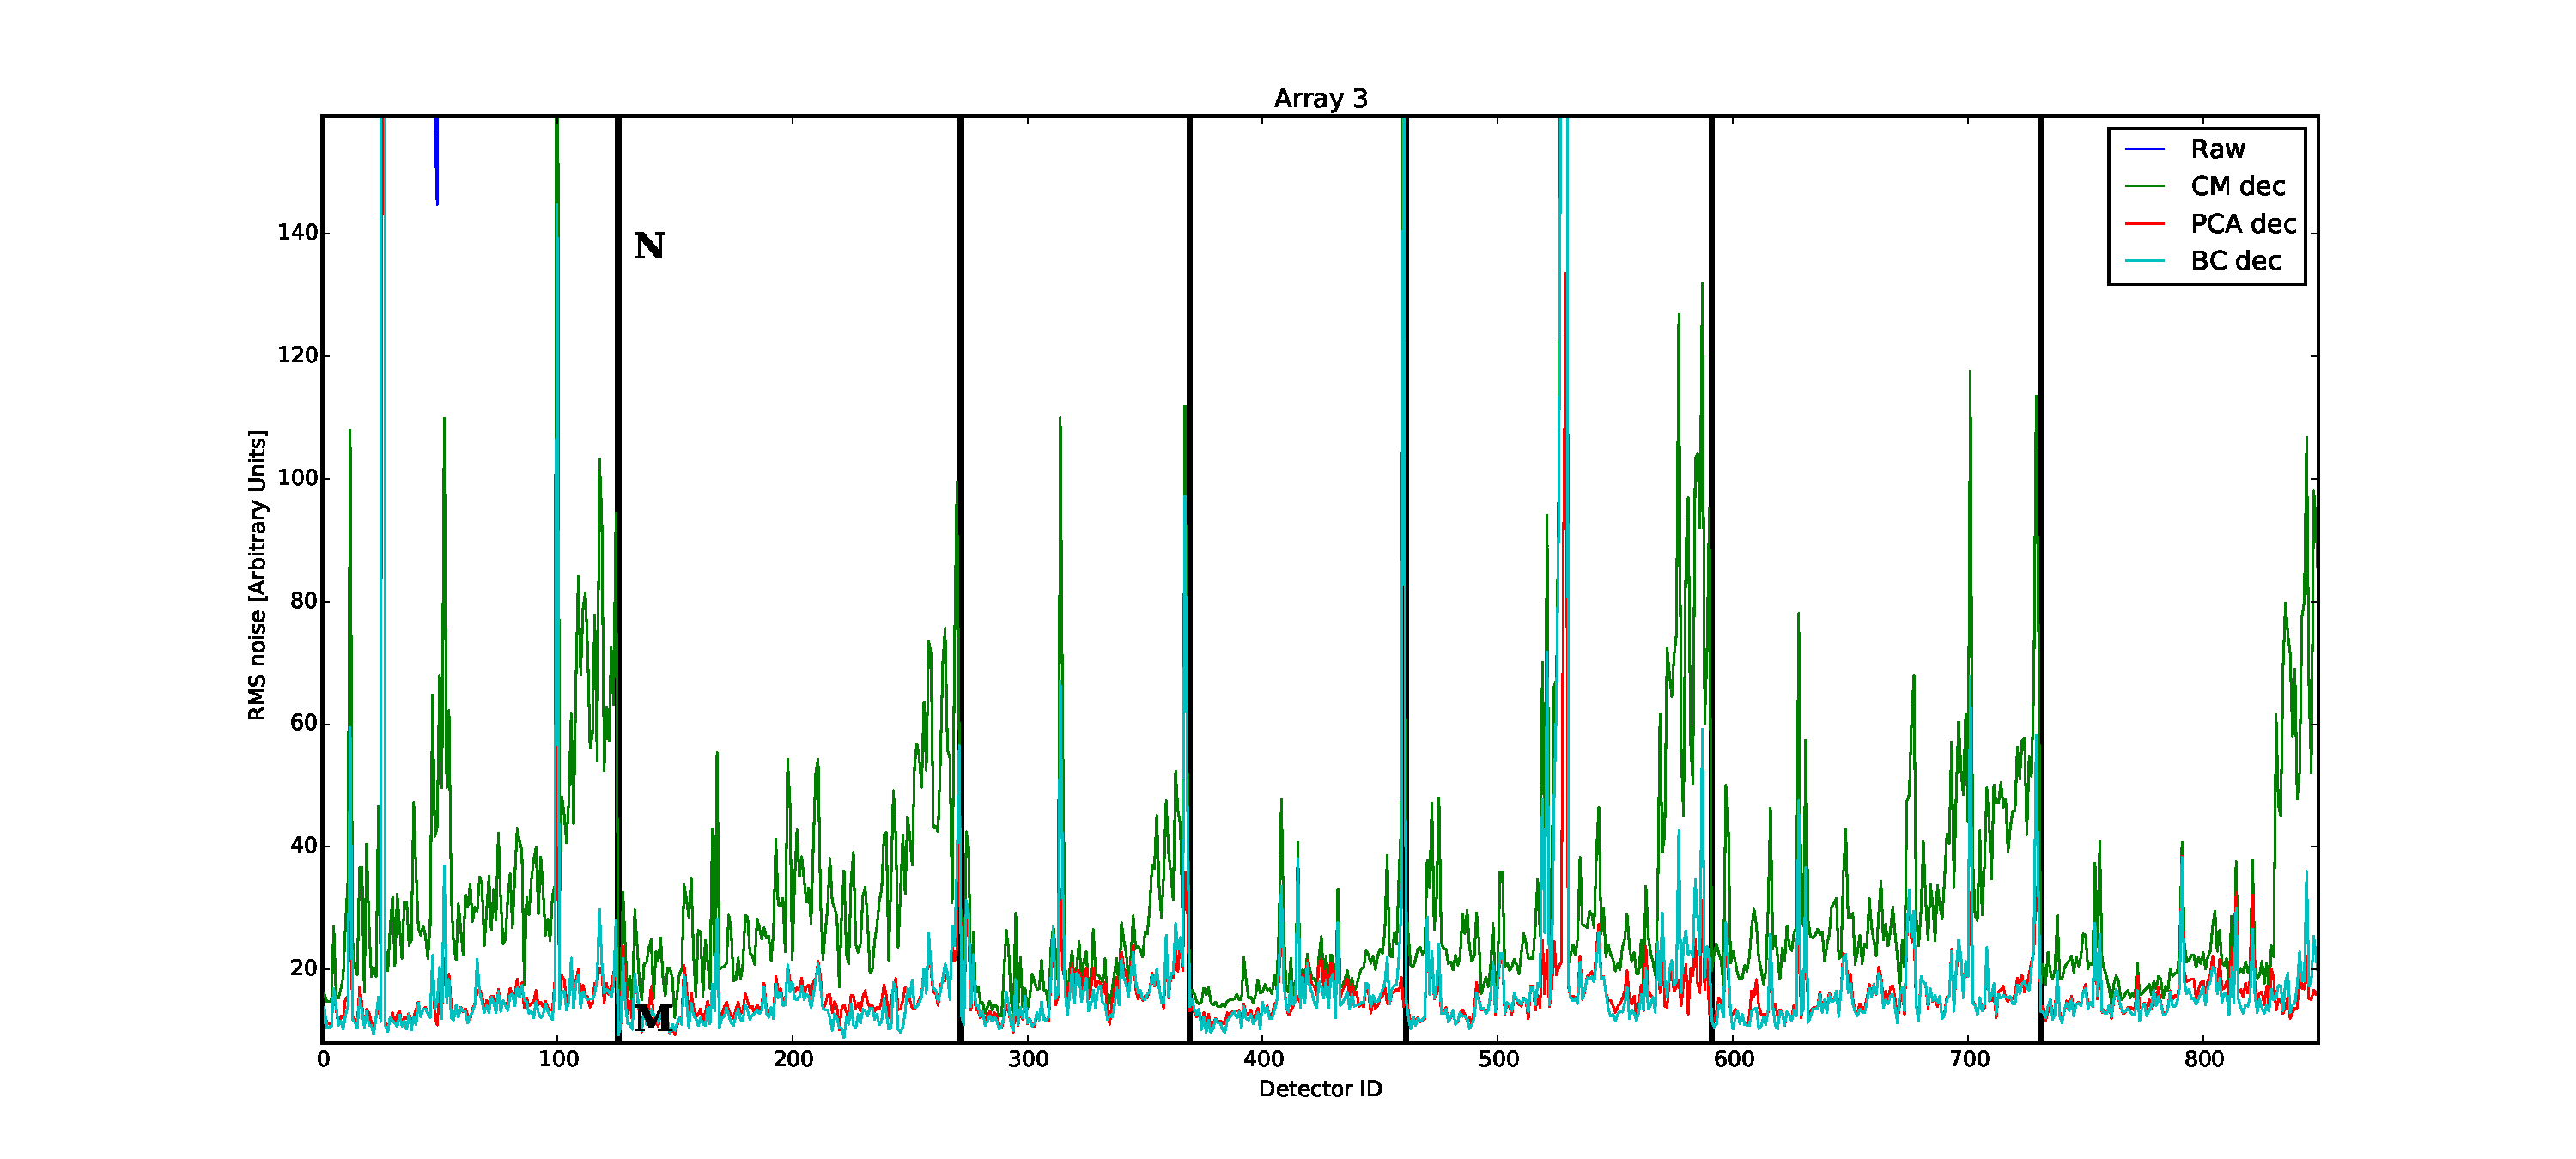
\includegraphics[clip=true, trim={0.5cm, 0, 0, 0.5cm},width=0.32\textwidth]{Figures/NoiseTests/rms_TOI_array_3_20170228s151.pdf}
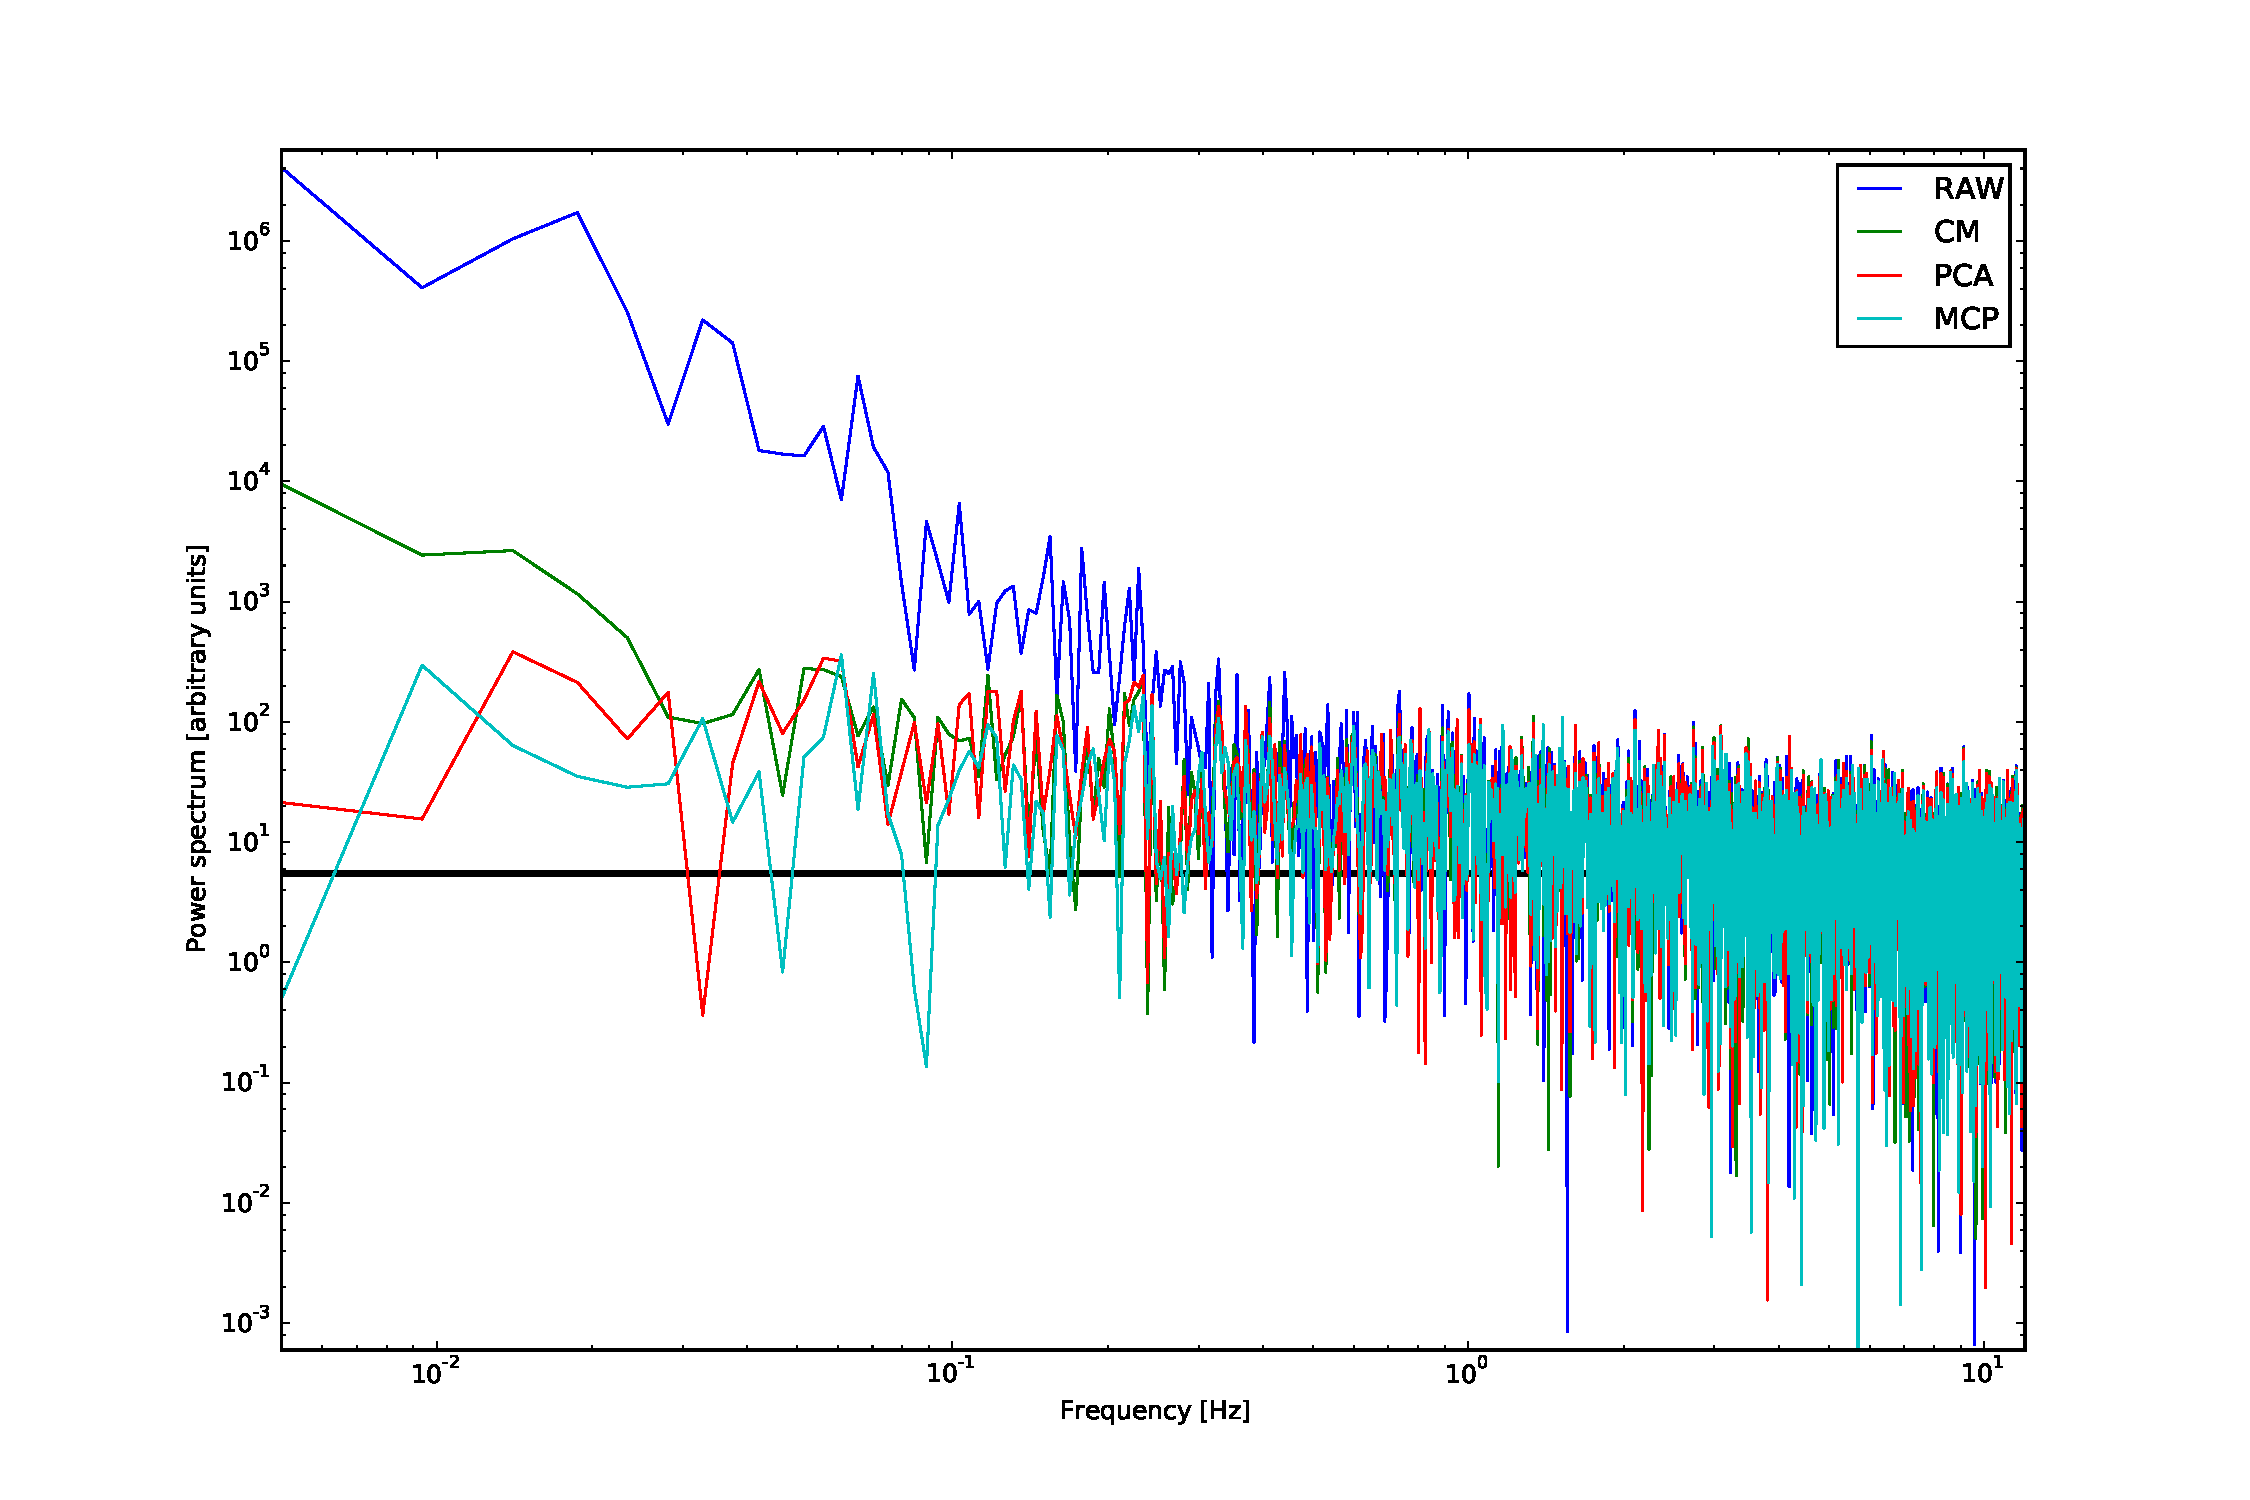
\includegraphics[clip=true, trim={0.5cm, 0, 0, 0.5cm},width=0.32\textwidth]{Figures/NoiseTests/pws_TOI_array_1_20170228s151.pdf}
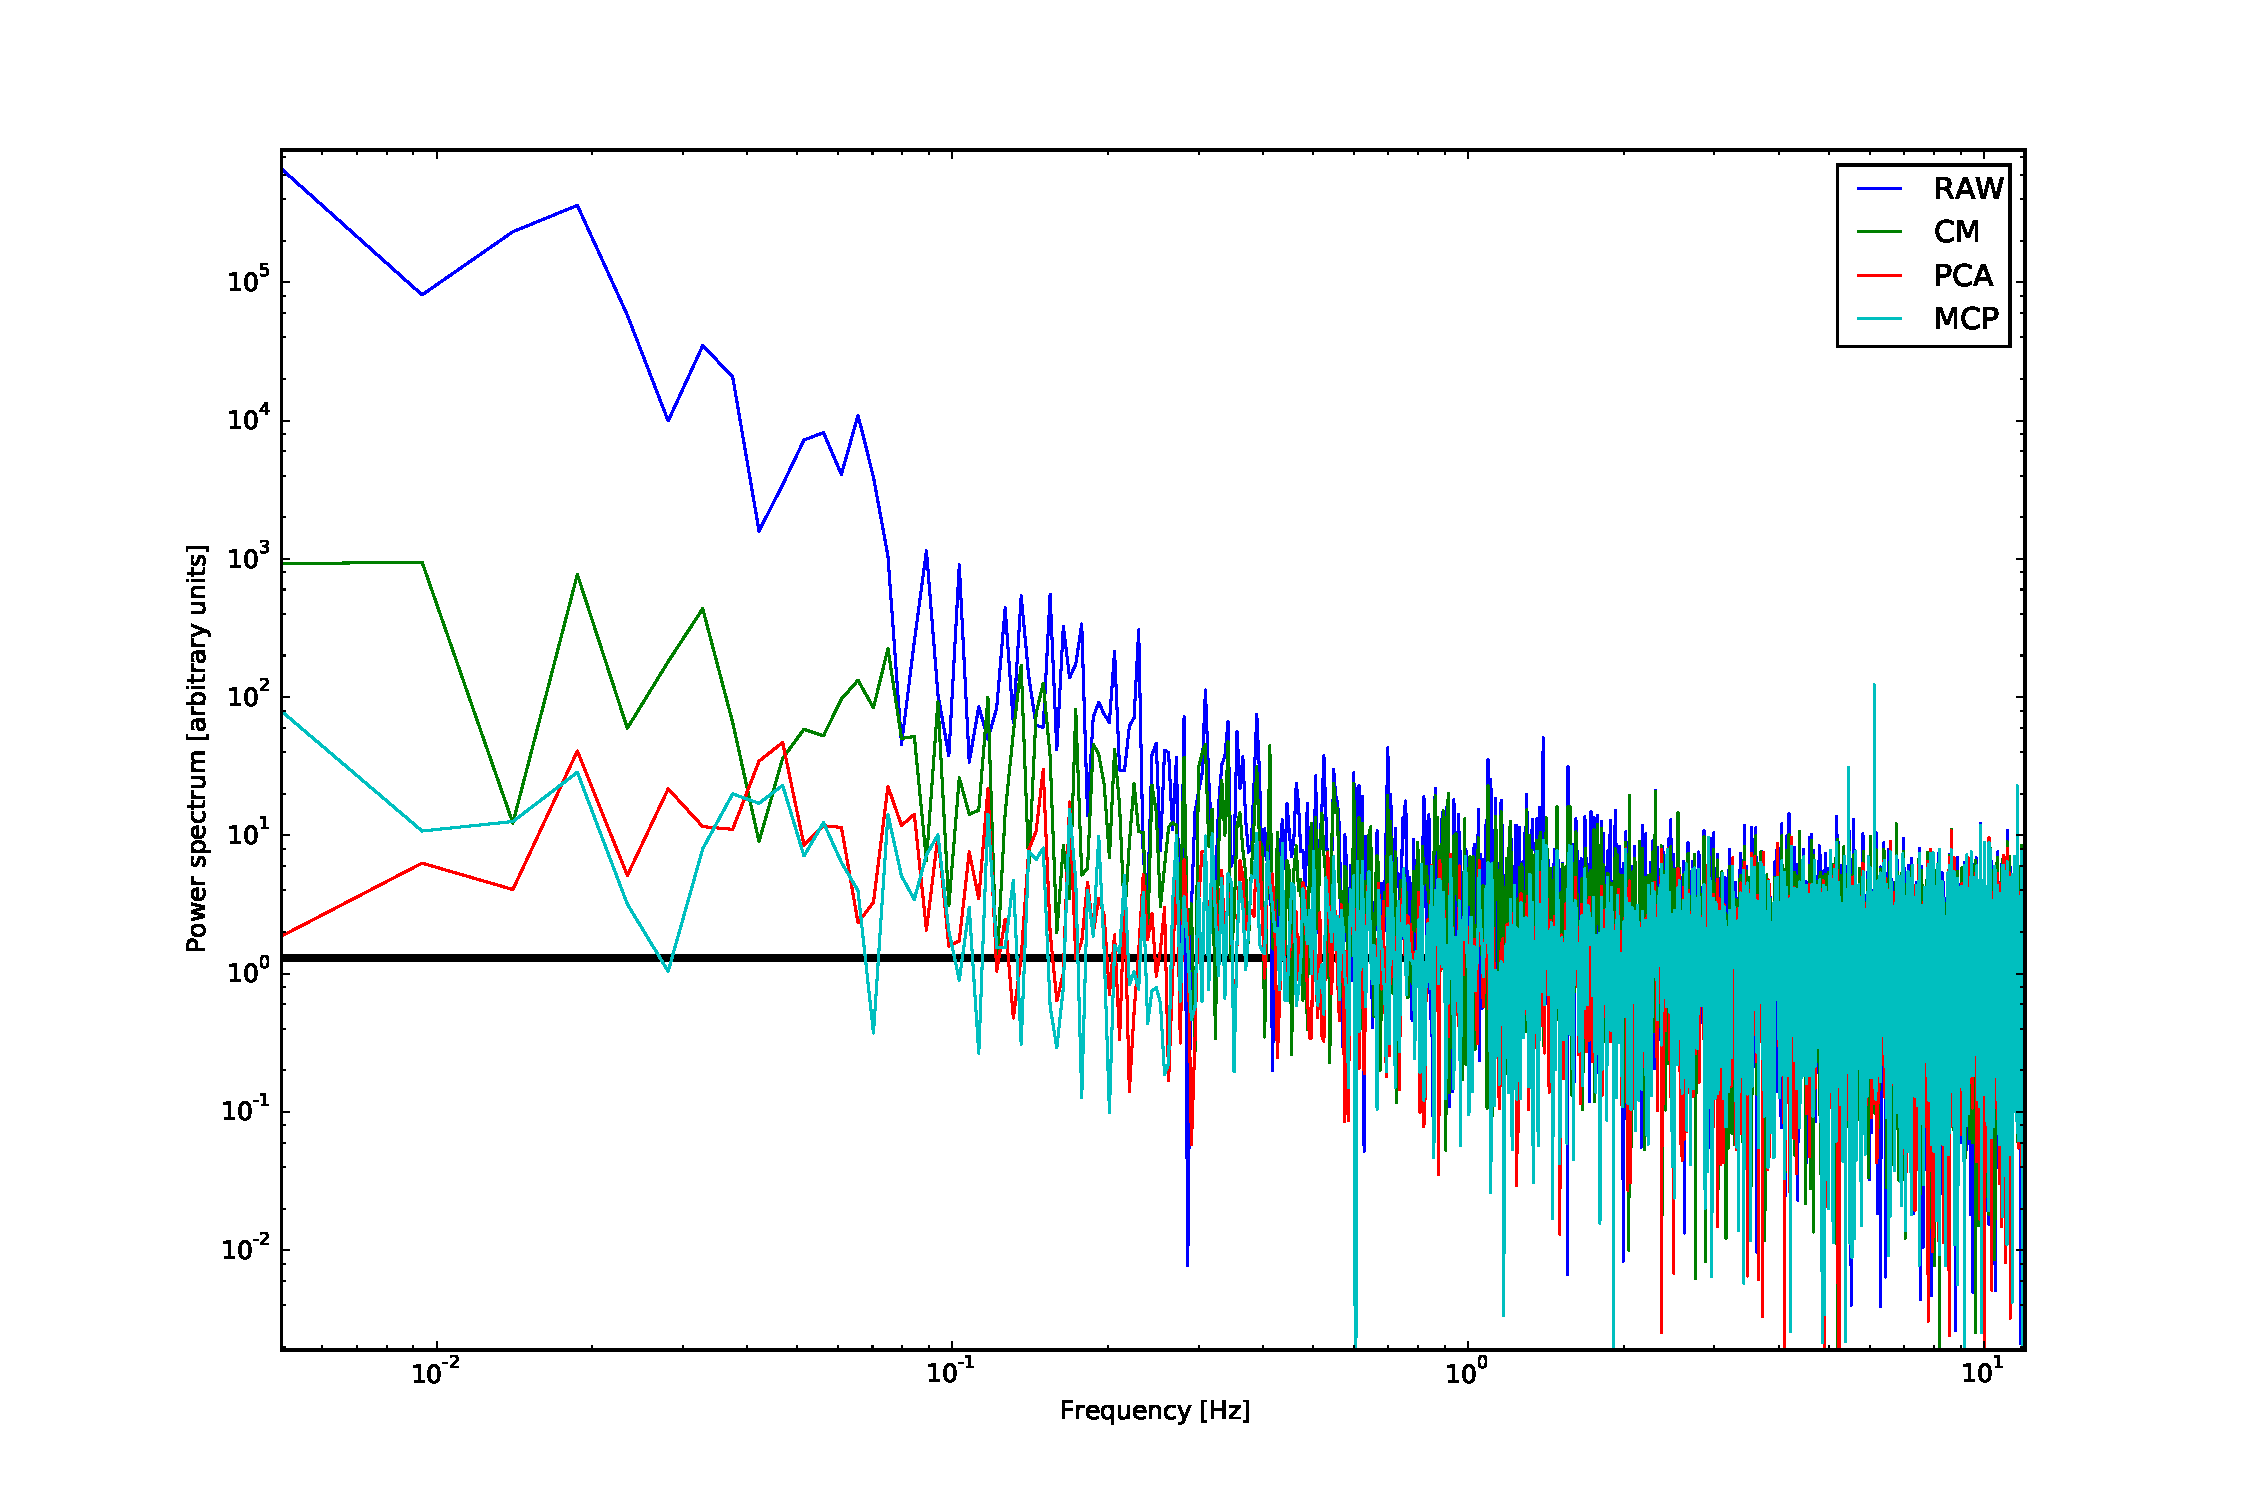
\includegraphics[clip=true, trim={0.5cm, 0, 0, 0.5cm},width=0.32\textwidth]{Figures/NoiseTests/pws_TOI_array_2_20170228s151.pdf}
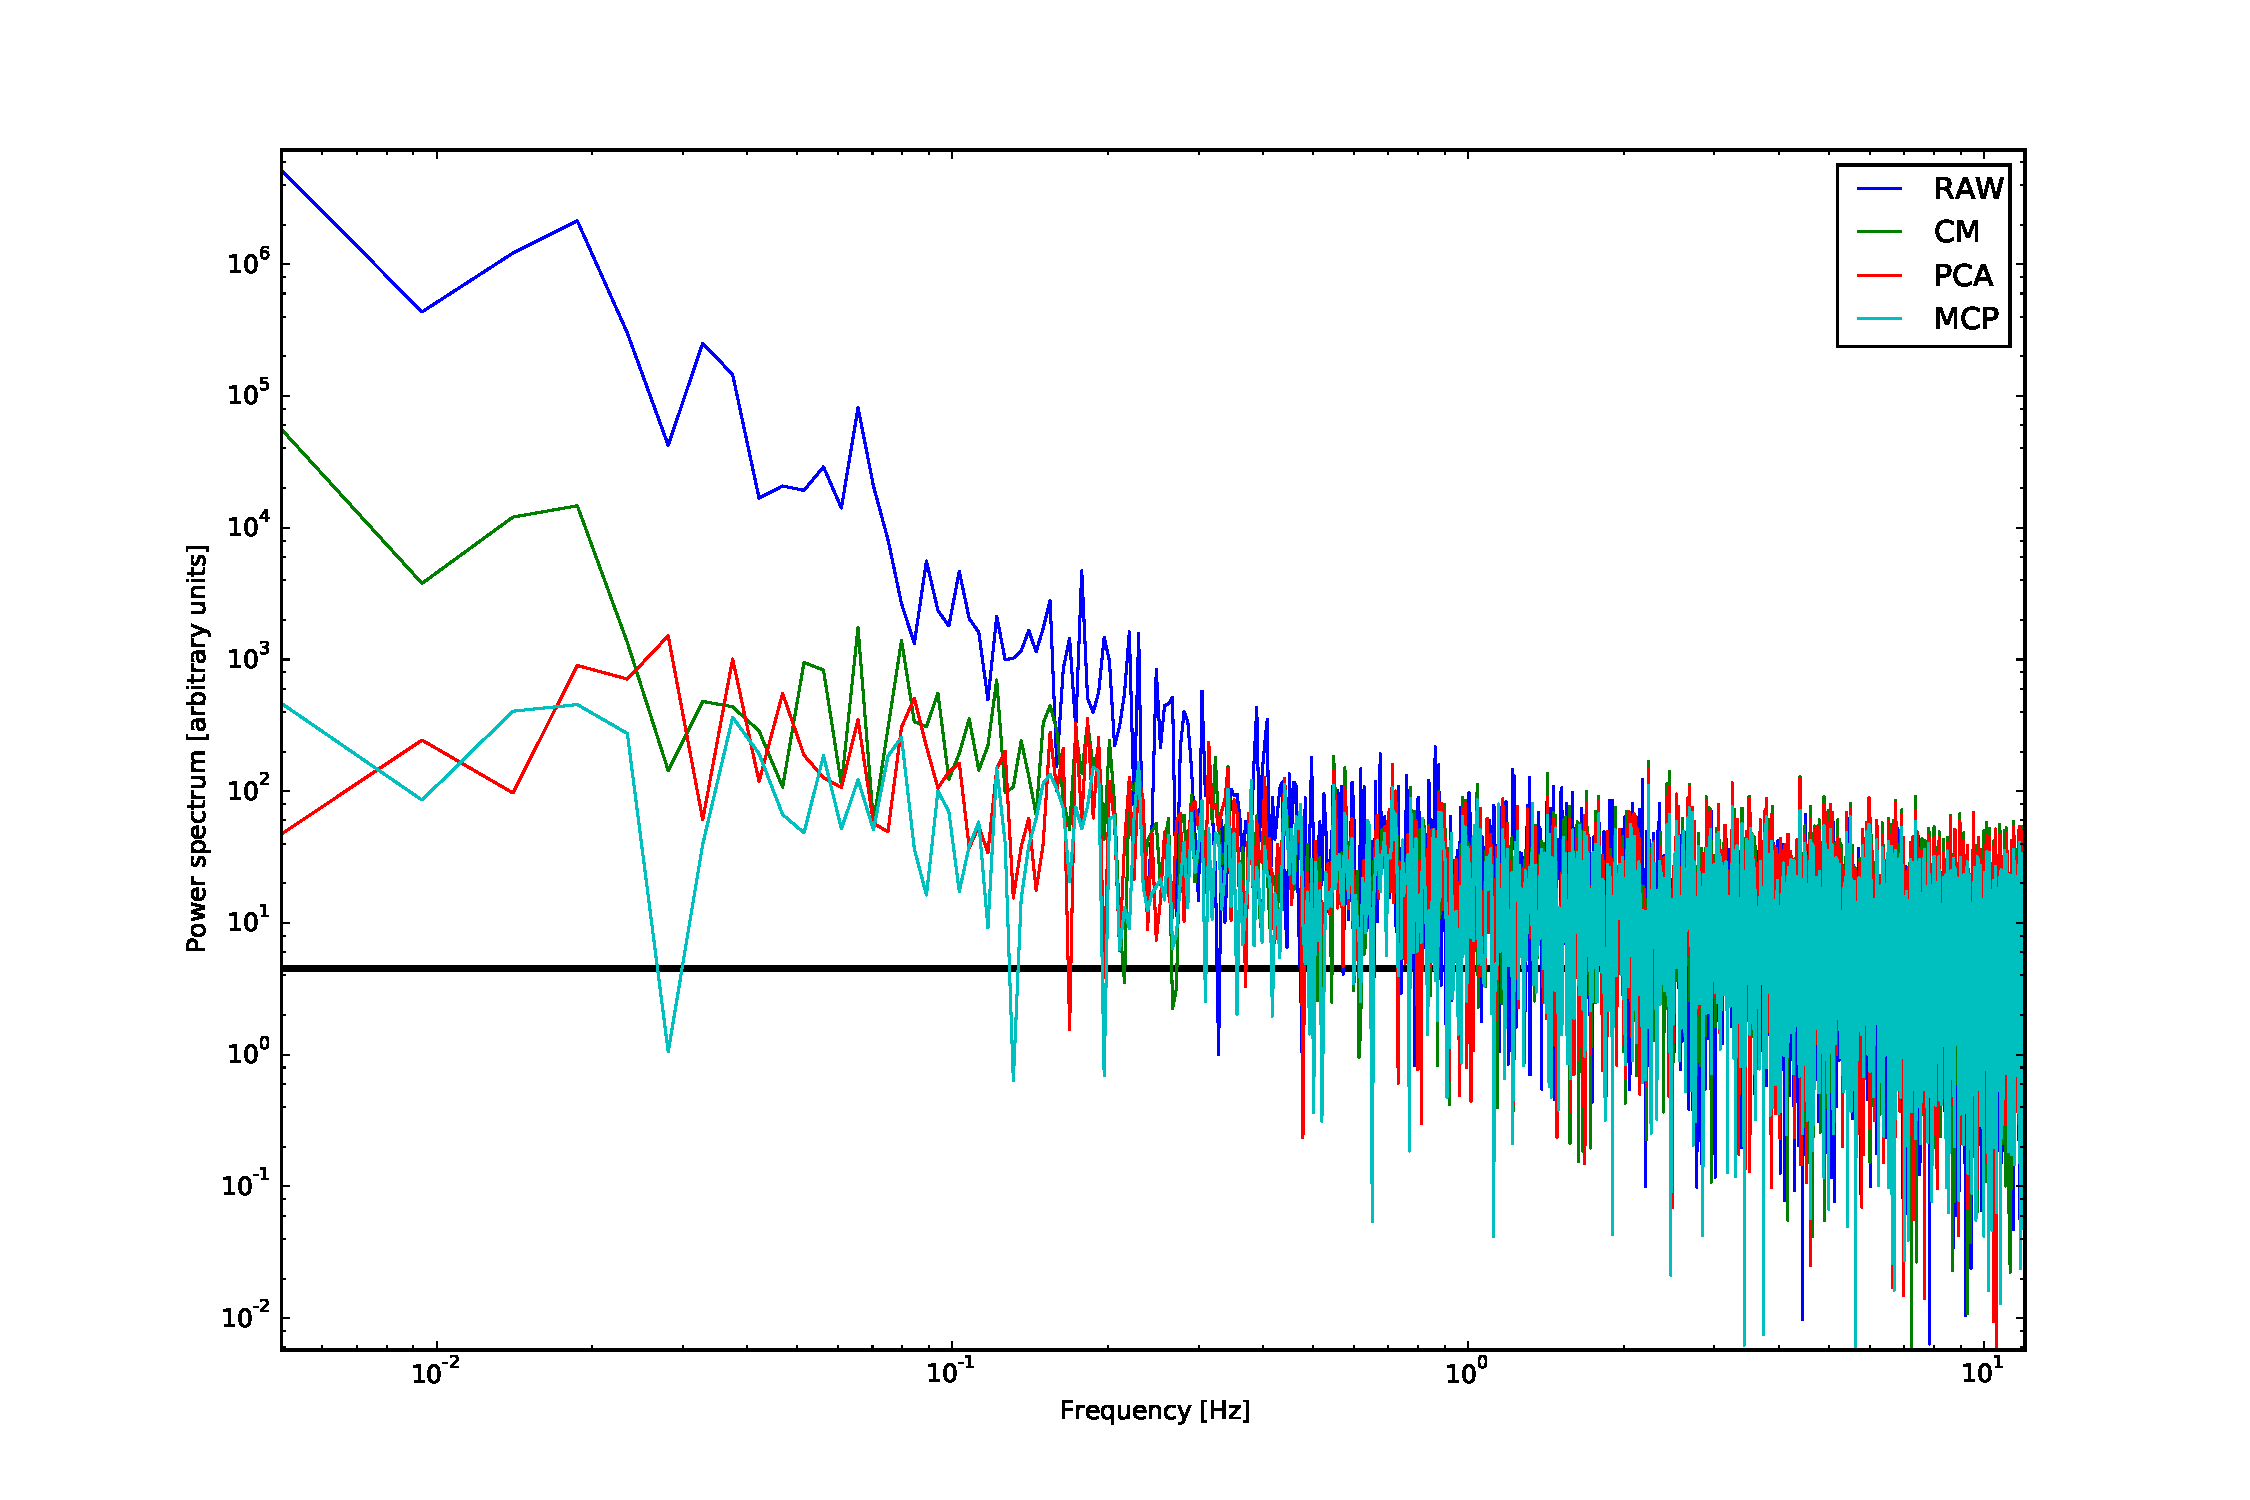
\includegraphics[clip=true, trim={0.5cm, 0, 0, 0.5cm},width=0.32\textwidth]{Figures/NoiseTests/pws_TOI_array_3_20170228s151.pdf}
\end{center}
\caption[Noise RMS and power spectra]{From top to bottom and from left to right,
  we show the data rms and power spectra for the three NIKA2 arrays (A1, A2, and
  A3) for scan 20170228s150. The rms and power spectra are given for the raw
  data (blue), and for the CM (green), PCA (red) and MCP (cyan) decorrelated
  data. The vertical lines in the rms noise figures separate detectors from
  different readout electronic boxes. Within each electronic box the pixels are
  ordered with increasing resonant frequency across the electronic
  band. \todo{To enlarge the y- and x- title}
  \label{rmspws}}
\end{figure}

In Fig.~\ref{rmspws} we present the rms noise per KID and the power spectra of
a typical raw datastream, and the CM, PCA and MCP decorrelated data. We observe that after
decorrelation we reduce significantly the rms of the
noise. Equivalently, the $1/f$-like noise in the power spectra
(principally due to atmospheric emission)
is significantly reduced leading to nearly flat spectra down to 0.05 Hz, with
larger $1/f$-like residual noise for the CM decorrelation method at lower
frequencies. This is translated into a larger rms noise for this method with
respect to the others. For the three arrays we find increasing noise with
increasing resonant frequency within each electronic box. This is probably
related to the difference of gains between subbands in the readout
electronics. We also find for the three arrays some noise bursts that are not
fully consistent from one decorrelation method to another. \\

We have investigated several ways of using this information to remove this
component from the TOIs. Our prefered choice so far, that is the reference
method for this document, is the \cmoneb\ method, that we describe into further
details below:

\begin{itemize}
\item From the pointing information (Sect.~\ref{se:ptg}), we derive a mask per TOI
  and for each time $t$ that is 0 if the KID is close to the source, 1
  otherwise. \new{In the case of a point source, the mask consists in 
    a radius of 60\,arcsec centered on the source, whereas for
    diffuse emission, tailored masks are build.}
\item Only samples for which two KIDs are far from the source,
  \new{hence which are not discarded using the mask,} are selected and the KID-to-KID
  correlation is computed.
  
\item For a KID $k_0$, we store the KID identifiers that are most
  correlated to it. We first select the 15 most correlated KIDs, then 
  the average and the dispersion $\sigma$ of these correlations are
  computed. \new{Then we add to the selection all the KIDs that are as correlated to $k_0$ as the
  15 first, up to $2\,\sigma$.}
\item A median common mode (far from the source) for this block of 15
  or more KIDs is derived. \todo{Marco's comment: How many ?}
\item A cross-calibration to each of these KIDs is computed using the
  median common mode. Then an inverse noise weighted average mode is build. At each time, we use
  only KIDs \new{that are not discarded with the source mask.} %that are further from the source than 60\,arcsec.
  At this stage it is important to verify to have enough KIDs to produce a
  continuous mode and to do not leave samples without any estimation.
\item We linearly regress this average mode against $k_0$'s TOI (far from the
  source) and subtract on the entire $k_0$ timeline.
\end{itemize}

This process is repeated for each KID. Fig.~\ref{fig:nika_toi} shows an example
of this low frequency mode derivation, together with the resulting TOI
cross-correlation matrix after its subtraction. We have tested on simulations
that this method does not alter the flux of the
source. \todo{Alessia's comment: Do we have a plot to show this ?}

If the observed field contains something else than a single point source at its
center, then several options are available to generalize this method. In
particular, the mask can be designed to adjust to several point sources. If the
source is diffuse and extended, then we may go through an iterative procedure that
subtracts an improved derivation of the signal at each step. For this work about
the commissioning of the instrument and the assessment of its performances on
point sources, we do not need to go into further details about this.

\subsection{Map projection}
\label{se:map_projection}

At this stage, data have been calibrated and cleaned and we have the pointing
information for each sample. If the noise was white and uncorrelated from KID to
KID, we would be able to produce an optimal map $S_p$ using an inverse
variance noise weighting of all of the measurements $m^k_t$ that fall
into a map pixel $p$ with a simple Nearest Grid Point procedure. In
this scheme, data samples are coadded with inverse variance noise
weighting: for each KID, we compute the standard deviation
$\sigma_k$ of its TOI far from the source (see Sect.~\ref{se:toi_proc}). Each
sample of this KID therefore has a weight of $1/\sigma_k^2$ and

\begin{eqnarray}
S_p        &=& \frac{1}{\sum_{k,t}1/\sigma_k^2}\sum_{k,t} \frac{m^k_t}{\sigma_k^2}\,, \label{eq:ngp_sum}\\
\sigma^2_p &=& \sum_{k,t}1/\sigma_k^2\,, \label{eq:ngp_var}
\end{eqnarray}

where $\sigma^2_p$ is the variance associated to pixel $p$. The
pipeline automatically projects one map per array and a combined 1\,mm
map and takes a small enough resolution to respect the Nyquist
criterion on the beam sampling.
To keep margin
and for the sake of simplicity, we usually take 2\,arcsec resolution pixels.

In practice, and although the data cleaning procedure described in
Sect.~\ref{se:toi_proc} significantly reduces the low frequency component of
TOIs, the residual noise is still not completely white nor KID independent. The
correlation matrix is not strictly zero to begin with (Fig.~\ref{fig:nika_toi})
and when looking at the distribution of the SNR on maps and variance maps
obtained with Eqs~(\ref{eq:ngp_sum},\ref{eq:ngp_var}), the distribution is
Gaussian, but not normalized to unity (see Fig.~\ref{fig:sigma_boost}). This is
due to the remaining correlations between TOIs before projection. At this stage,
rather than putting more effort in TOI processing, we renormalize the width of
the Gaussian noise, which actually increases the map variance by the required factor
so that the SNR distribution becomes normalized. This normalization factor
varies from scan to scan but it is usually between 1.2 and 1.5. It is estimated on
the background of the map, i.~e. far from the source.

\begin{figure}[ht!]
\begin{center}
\includegraphics[clip, angle=0, scale=1, width=0.75\textwidth]{Figures/sigma_boost.eps}
\caption[Distribution of the SNR per beam]{Histogram of the SNR per beam on a scan of weak source (G2, see
  Sect.~\ref{se:nefd_estimation_methods}). While the histogram is Gaussian, its
  width is not normalized to 1 due to residual correlated noise between the
  TOIs. This factor is accounted for before delivering the final variance map
  and associated flux estimates.}
\label{fig:sigma_boost}
\end{center}
\end{figure}

When several scans of the same source are averaged, we apply an inverse
variance weighting as well. Weights are taken from the variance maps of each scan,
corrected for the excess variance mentioned in the previous paragraph. The
final variance map of the sum of scans is also corrected for such a factor if necessary.

\subsection{Photometry}
\label{se:intro_photometry}

Throughout this document, we adopt the following convention. Assuming the beam
is a perfect Gaussian of known $FWHM=\sigma\sqrt{8\ln 2}$, the instantaneous
signal measured by a KID is

\begin{equation}
m^k(x,y) = \phi e^{-(x^2+y^2)/2\sigma^2} = \phi G(x,y)
\label{eq:flux_per_beam_def}
\end{equation}

with $\phi$ the flux of the source \new{and $(x,\, y)$ the coordinates in
the chosen system.} In practice, the beam is not a perfect Gaussian
and significant side lobes must be accounted for
(Sect.~\ref{se:beams}). If the beam was perfectly known and stable, we could in
principle replace the Gaussian form in Eq.~\ref{eq:flux_per_beam_def} by the
beam pattern and fit for the amplitude $\phi$. In practice, we have found that
it was enough as a first approximation to take an equivalent effective Gaussian
width and use it to derive the beam template. We take 12.5 and 18.5\,arcsec FWHM
at 1 and 2\,mm respectively and compute all our fluxes with these
values. We do this for both analyzed point sources and for absolute calibrators
to be consistent. Our photometric system is further detailed in
Sects.~(\ref{se:cal_HA_reference}, \ref{se:cal_HA_main}). 

Let's call $s_p$ the measured signal at map pixel $p$ and denote by $g_p$ the
Gaussian weight given to pixel $p$ as a function of its distance to the source,
as defined in Eq.~\ref{eq:flux_per_beam_def}. The amplitude fit is performed
with an usual maximum likelihood approach. We assume that the renormalization of
the variance map described in the previous section is enough to account for the
residual noise correlations from pixel to pixel and therefore assume the pixels to
be independent in this estimator:

\begin{eqnarray}
\hat{\phi} &=& \frac{1}{\sum_p g_p^2/\sigma_p^2}\sum_p
s_p\frac{g_p}{\sigma_p^2} \label{eq:flux_estim_def} \\
\sigma^2(\hat{\phi}) &=& \frac{1}{\sum_p
  g_p^2/\sigma_p^2} \label{eq:flux_estim_var_def}
\end{eqnarray}

In the case of Gaussian white noise, this maximum likelihood estimator coincides
with the classical minimum variance estimator and thus provides the best SNR
estimate of the source flux.

%% \subsection{Opacity correction}
%% 
%% Water vapor along the line of sight absorbs power from the source and therefore
%% biases the flux measurement. At the same time, the overall airmass acts as a
%% diffuse source of power on the KIDs that induce a variation of their resonance
%% frequency. We are able to calibrate it and therefore derive the opacity in real
%% time from \nika\ data. This is described in details in
%% Sect.~\ref{se:opacities}. Suffice is here to say that after the derivation of
%% the KID offsets and their relative gains as described in
%% Sect.~\ref{se:fov_first_geometry}, one we know the opacity, we can derive an
%% absolute calibration per KID.

%% \subsection{Absolute calibration}
%% \todo{See how to talk about Planet models and repeated observations of these to derive
%% the ``final'' abs. cal for the run.}
%% 
%% %The data reduction of \nika\ cannot be done exclusively KID by KID
%% %independently. Each matrix is a filled array with more than one detector per PSF
%% %and the atmosphere together with the electronics chain act as correlated
%% %noise. We therefore have to work iteratively to improve both individual and
%% %global parameters of the detectors. In this section, we give an overview of the
%% %full data reduction that illustrates this iterative process. More details on
%% %each specific step are given in other dedicated sections.
%% 
%% \subsection{Overview of the on-sky calibration method}
%% 
%% The steps to go from raw timeline data in Hertz to calibrated data in Jansky per beam comprize:
%% \begin{itemize}
%% \item[] Opacity correction
%% \item[] Field-of-view geometry and KIDs selection
%% \item[] KID-to-KID intercalibration (flat fielding)
%% \item[] Absolute calibration  
%% \end{itemize}
%% 
%% 
%% \subsection{Data reduction summary {\color{blue} Nico}}
%% 
%% The performance assessment relies on a data reduction pipeline that consists of the following steps:
%% \begin{itemize}
%% \item[] reading of the raw timeline 
%% \item[] implementation of the calibration
%% \item[] substraction of the correlated part of the noise 
%% \item[] projection of the timeline onto maps
%% \end{itemize}
